
\documentclass[preprint,12pt]{elsarticle}





\usepackage{amsmath,amssymb,amsfonts,stmaryrd,amsthm}
\usepackage{graphicx}
\usepackage{pstricks}
\usepackage{algorithm}
\usepackage{algorithmic}

\hyphenation{English}





\journal{Journal of Computational and Applied Mathematics}

\newtheorem{theorem}{Theorem}[section]
\newtheorem{assumption}[theorem]{Assumption}
\newtheorem{lemma}[theorem]{Lemma}

\newcommand{\pe}{\psi}
\def\d{\delta} 
\def\ds{\displaystyle} 
\def\e{{\epsilon}} 
\def\eb{\bar{\eta}}  
\def\enorm#1{\|#1\|_2} 
\def\Fp{F^\prime}  
\def\fishpack{{FISHPACK}} 
\def\fortran{{FORTRAN}} 
\def\gmres{{GMRES}} 
\def\gmresm{{\rm GMRES($m$)}} 
\def\Kc{{\cal K}} 
\def\norm#1{\|#1\|} 
\def\wb{{\bar w}} 
\def\zb{{\bar z}} 

\def\qed{Q.E.D.}

\newtheorem{definition}[theorem]{Definition}

\newcommand{\cS}{\mathcal{S}}
\newcommand{\tU}{\tilde{U}}
\newcommand{\ta}{\tilde{a}}
\newcommand{\tk}{\tilde{k}}
\newcommand{\bfb}{\mathbf{b}}
\newcommand{\tB}{\tilde{\mathcal{B}}}
\newcommand{\cV}{\mathcal{V}}
\newcommand{\cT}{\mathcal{T}}
\newcommand{\calB}{\mathcal{B}}
 \newcommand{\cB}{{B}}
\newcommand{\cL}{\mathcal{L}}
\newcommand{\cK}{\mathcal{K}}
\newcommand{\cE}{\mathcal{E}}
\newcommand{\cI}{\mathcal{I}}
\newcommand{\cA}{{A}}
\newcommand{\calA}{\mathcal{A}}
\newcommand{\cO}{\mathcal{O}}
\newcommand{\osc}{\mathrm{osc}}
\newcommand{\R}{\mathbb{R}}
\newcommand{\N}{\mathbb{N}}
\newcommand{\bk}{\mathbf{k}}
\newcommand{\br}{\mathbf{r}}
\newcommand{\tcb}{\textcolor{blue}}


\def\bfE{\mbox{\boldmath$E$}}
\def\bfG{\mbox{\boldmath$G$}}


\begin{document}

\begin{frontmatter}



\title{An Iterative Adaptive Finite Element Method\\ for Non-Symmetric Elliptic Eigenvalue Problems}


\author[aut1]{Pavel~Solin}
\ead{solin@unr.edu}

\author[aut2]{Stefano~Giani\corref{cor1}}
\ead{stefano.giani@nottingham.ac.uk}

\cortext[cor1]{Corresponding author}

\address[aut1]{Department of Mathematics and Statistics, University of Nevada, Reno, USA, and Institute of Thermo-mechanics,
Prague, Czech Republic}

\address[aut2]{School of Mathematical Sciences
University of Nottingham , University Park, Nottingham, NG7 2RD,  United Kingdom,
Phone: +44 (0) 115 8467916}

\begin{abstract}


\end{abstract}

\begin{keyword}
partial differential equation \sep eigenvalue problem \sep iterative method \sep
adaptive higher-order finite element
method \sep $hp$-FEM \sep reproducible research
\MSC 65N25 \sep 65N30 \sep 65N50 \sep 35B45
\end{keyword}

\end{frontmatter}



\begin{abstract}

\end{abstract}




\section{Introduction}\label{sec:intro}
\setcounter{equation}{0}

We have to assume that the model problem is a diagonalizable non-symmetric differential operator.
Pavel, this is important otherwise when could not have eigenvalues. 

Model problem:
\begin{equation} \label{one}
-\Delta u + b\cdot\nabla u + cu = \lambda u, \ \ \ u = 0 \ \mbox{on} \ \partial \Omega
\end{equation}
where 
$b \in \big[L^\infty(\Omega)\big]^2$ and $c\in L^\infty(\Omega)$ is non-negative.


\subsection{Outline of the Paper}



\section{Motivation}\label{sec:motiv}

This work is motivated by the fact that non-symmetric eigenvalue problems have in general have very different left and right eigenfunctions for the same eigenvalue.
In Figure~\ref{fig:eigen1} we reported the left and right eigenfunctions corresponding to the smallest eigenvalue of problem \eqref{one} on the unit sqaure with $b:=(5,5)$ and $c:=0$. 
As can be seen the two functions are different and in particular most of the energy of the modes is concentrated in different regions. It is straightforward to conclude that this two eigenfunctions can not be approximated efficiently using the same sequence of adapted meshes for both of them. For this reason we developed the methods presented in this work that use two independent sequences of refined meshes to approximate the left and right eigenfunctions.
In Figure~\ref{fig:mesh1} we reported the $hp$-adapted meshes for the eigenfunctions in Figure~\ref{fig:eigen1}.

\begin{figure}[!ht]
\begin{center}
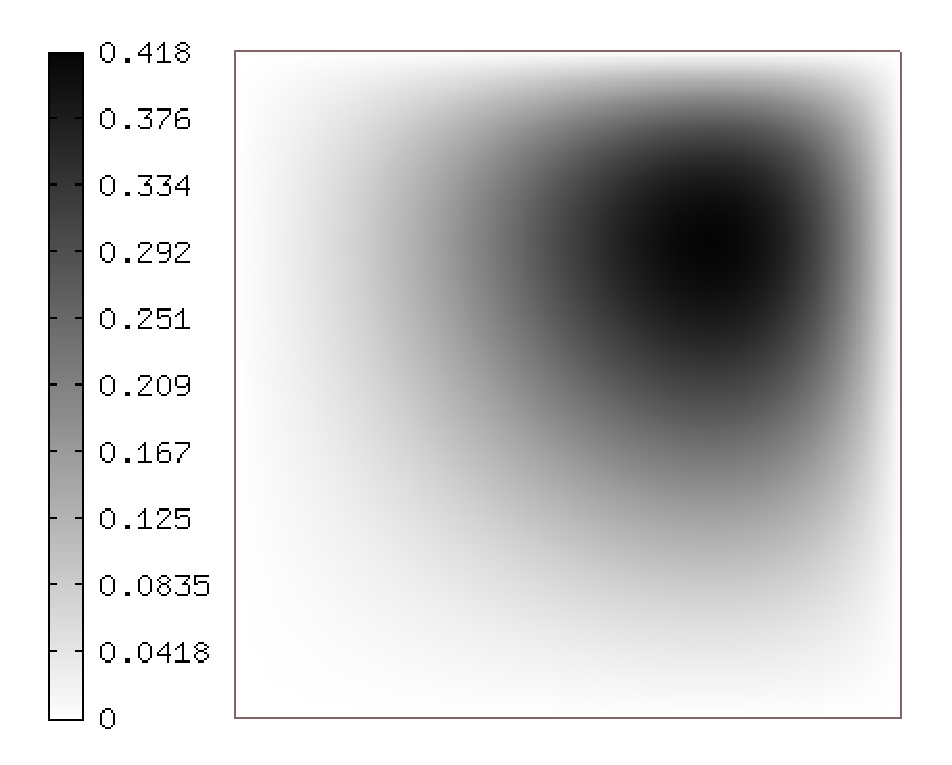
\includegraphics[width=0.4\textwidth]{eig1.eps}\ \ \ 
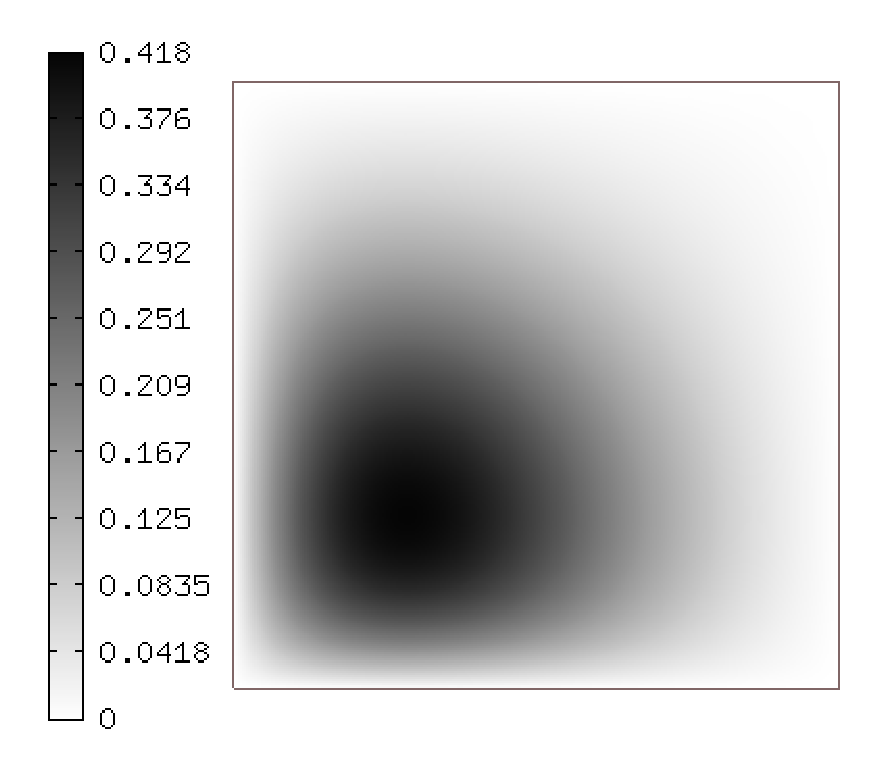
\includegraphics[width=0.4\textwidth]{eig2.eps}\\
\end{center}
%\vspace{-5mm}
\caption{Left and right eigenfunctions corresponding to the smallest eigenvalue of problem \eqref{one}. }
\label{fig:eigen1}
\end{figure}

\begin{figure}[!ht]
\begin{center}
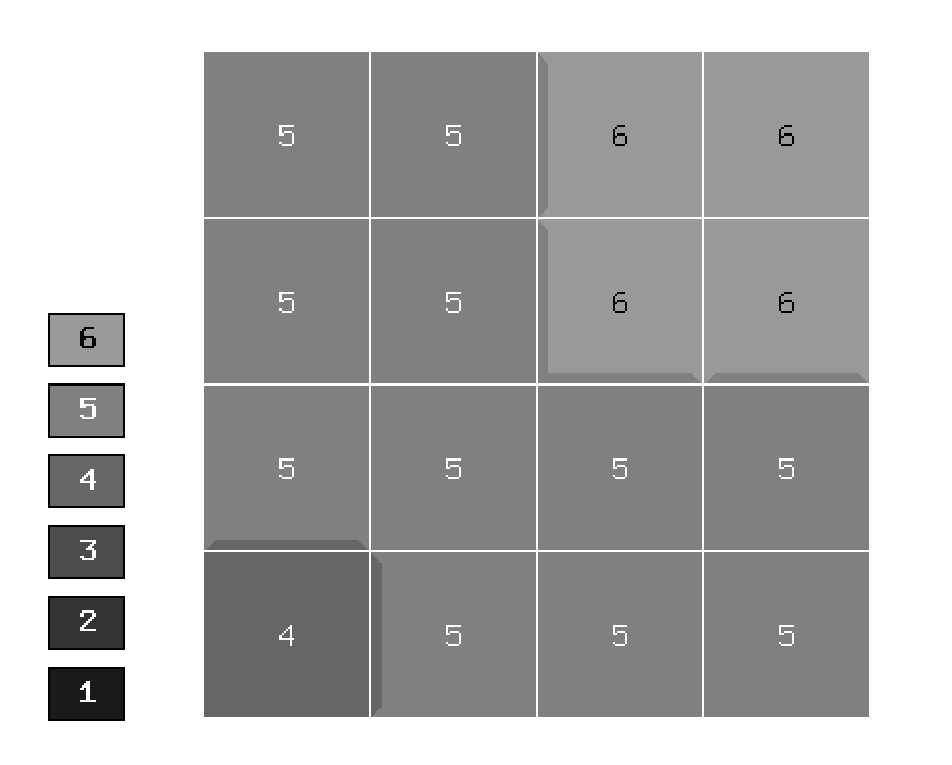
\includegraphics[width=0.4\textwidth]{mesh1.eps}\ \ \ 
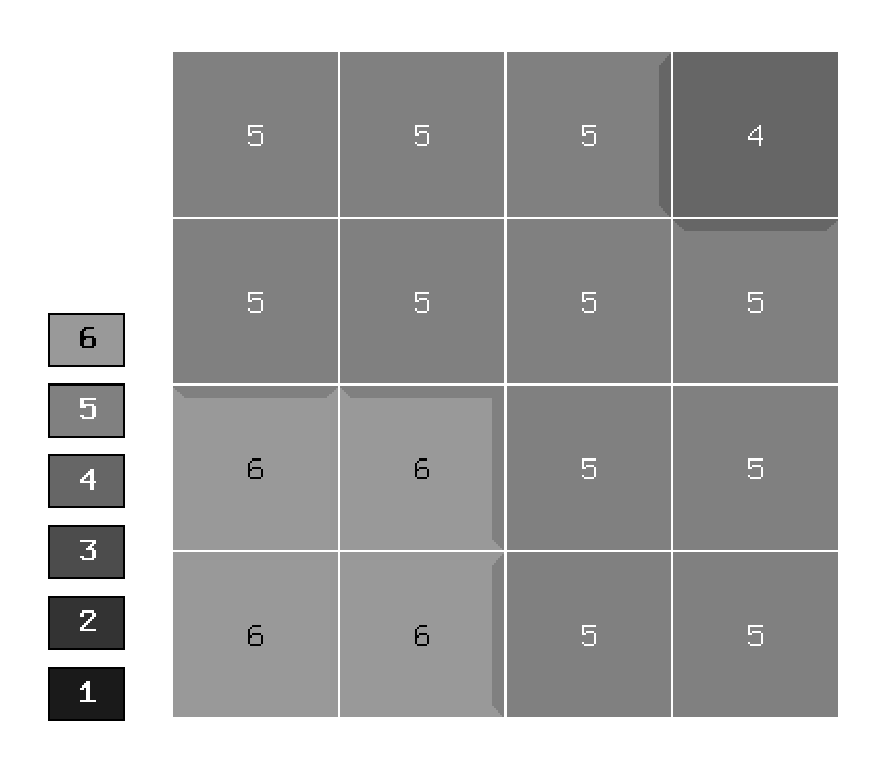
\includegraphics[width=0.4\textwidth]{mesh2.eps}\\
\end{center}
%\vspace{-5mm}
\caption{$hp$-adapted meshes for the left and right eigenfunctions in Figure~\ref{fig:eigen1}. }
\label{fig:mesh1}
\end{figure}



%%%%%%%%%%%%%%%%%%%%%%%%%%%%%%%%%%%%%%%%%%%%%%%%%%%%%%%%%%%%%%%%%%%%%%%%%%%%%%%%%%%%%%%%%%%%%%%%%%%%%%%%%

\section{Preliminaries}\label{sec:preli}

Throughout, $L^2(\Omega)$
denotes the usual space of square-integrable real valued functions
equipped with the standard norm
\begin{equation}\label{eq:l2}
\|f\|_{0}\ := \ \left(\int_\Omega  |f|^2\right)^{\frac{1}{2}} .
\end{equation}
The symbol $H^1(\Omega)$ denotes the usual space of functions in $L^2(\Omega)$
with square-integrable weak first partial derivatives. The $H^1$-norm is 
denoted by $\|f\|_1$.

Since problem \eqref{one} is non-symmetric, we have that in general for the same eigenvalue the left and the right eigenfunctions are different. So it is reasonable to compute for each eigenvalue both corresponding eigenfunctions, i.e. $(\lambda_j,u_j,u_j^*)\in \mathbb{R}\times E(\lambda_j)\times E^*(\lambda_j)$, where $E(\lambda_j)$ and $E^*(\lambda_j)$ are respectively the left and right eigenspaces.
The variational formulation for the left eigenfunction of problem \eqref{one} is:
\emph{Find the eigenvalue $\lambda_j\in \mathbb{R}$ and the eigenfunctions $u_j,u_j^*\in H^1_0(\Omega)$
such that}
\begin{equation}
\label{eq:var_prob}
\left.
\begin{array}{lcl}
a(u_j,v)&=& \lambda_j\ b(u_j,v),
\quad \text{for all } \quad v  \in H^1_0(\Omega)\\
a(v,u_j^*)&=& \lambda_j\ b(v,u_j),
\quad \text{for all } \quad v  \in H^1_0(\Omega)\\
 b(u_j,u_j^*) &=& 1
\end{array}\quad
\right\}
\end{equation}
where
\begin{equation}\label{eq:a}
a(u,v):=\int_\Omega \nabla u(x)\cdot \nabla v(x) + b\cdot \nabla u(x) v(x) + cu(x)v(x),
\end{equation}
and
\begin{equation}\label{eq:b}
b(u,v):=\int_\Omega u(x) v(x).
\end{equation}



Because the left and the right eigenfunctions can be very different, we use two sequences of meshes, one for each eigenfunction, and we apply adaptivity to each eigenfunction independently. 
To discretize (\ref{eq:var_prob}), let $\cT_n, n =
1,2,\ldots $ denotes a family of meshes on $\Omega$.
The meshes can be irregular with multiple levels of hanging nodes, 
and they can combine possibly curvilinear triangular and quadrilateral 
elements. These meshes may be obtained using automatic adaptivity. 
Similarly for the right eigenfunctions we use irregular mesh of the same kind,  $\cT_n^*, n =
1,2,\ldots $ denote a family of meshes on $\Omega$.

In the rest of the paper we are going to denote with a star all quantities related to the right eigenfunction.

By $h_{n,\tau}$ we denote the diameter of element $\tau$,  
we define
$
h_n:=\max_{\tau\in \mathcal{T}_n}\{h_{n,\tau}\}.
$
Similarly with  $p_{n,\tau}$ we denote  the order of polynomials of element $\tau$,  
we define
$
p_n:=\min_{\tau\in \mathcal{T}_n}\{p_{n,\tau}\}.
$
On any mesh $\mathcal{T}_n$ we denote by $V_n \subset H^1_0(\Omega)$ the finite
dimensional space of continuous functions $v$ such that on any element $\tau$ we 
have that $v|_\tau\in \mathcal{P}_{p_{n,\tau}}(K)$. Here either $\mathcal{P}_{p_{n,\tau}}(K)$ 
is the space of polynomials of total degree at most $p_{n,\tau}$ if $\tau$ is a triangular 
element, or $\mathcal{P}_{p_{n,\tau}}(K)$ is the space of polynomials of degree at most 
$p_{n,\tau}$ in each variable if $\tau$ is a quadrilateral element.



The discrete version of \eqref{eq:var_prob} reads:
\emph{Find the eigenvalue $\lambda_{j,n}\in \mathbb{R}$ and the eigenfunctions $u_{j,n}\in V_n$ and $u_{j,n}^*\in V_n^*$
such that}
\begin{equation}
\label{eq:disc_prob}
\left.
\begin{array}{lcl}
a(u_{j,n},v_{n})&=& \lambda_{j,n}\ b(u_{j,n},v_{n}),
\quad \text{for all } \quad v_{n}  \in V_n\\
a(v_{n},u_{j,n}^*)&=& \lambda_{j,n}\ b(v_{n},u_{j,n}^*),
\quad \text{for all } \quad v_{n}  \in V_n^*\\
 b(u_{j,n},u_{j,n}^*) &=& 1
\end{array}\quad
\right\}
\end{equation}

The methods presented in this work make use of a third sequence of meshes $\mathcal{T}_n^U$ which, for each $n$, $\mathcal{T}_n^U$ is the union of the two meshes  $\mathcal{T}_n$ and $\mathcal{T}_n^*$. Similarly we define the spaces $V_n^U$ constructed on the meshes $\mathcal{T}_n^U$ which contain the spaces $V_n$ and $V_n^*$ for each $n$. 

\textcolor{red}{Pavel, can you explain better how this thing about the union of the meshes and the common FE space works?}

Then for any function $v\in V_n$ we can defined a trivial prolongation operator $P$ such that $Pv\in V_n^U$ is the prolongation of $v$ in $V_n^U$ and similarly we can define the trivial prolongation operator $P^*$ from $V_n^*$ into $V_n^U$. %Let also denote the restriction operators $R:V_n^U\rightarrow V_n$ and $R^*:V_n^U\rightarrow V_n^*$ satisfying for $v\in V_n$ $v\equiv RPv$ and for $v\in V_n^*$ $v\equiv R^*P^*v$.

%%%%%%%%%%%%%%%%%%%%%%%%%%%%%%%%%%%%%%%%%%%%%%%%%%%%%%%%%%%%%%%%%%%%%%%%%%%%%%%%%%%%%%%%%%%%%%%%%%%%%%%%%

\section{Picard's Method}\label{sec:picard}

Problem \eqref{eq:disc_prob} can be reformulated in matrix form as:
\emph{Find an eigenvalue $\lambda\in \mathbb{R}$ and an eigenvectors $\mathbf{u}\in \mathbb{R}^N$, where $N$ is the dimension of $V_n$ and $\mathbf{u}^*\in \mathbb{R}^{N^*}$, where $N^*$ is the dimension of $V_n^*$,
such that}
\begin{equation}
\label{eq:disc_prob_mat}
\left.
\begin{array}{lcl}
\mathbf{A} \mathbf{u}&=& \lambda\mathbf{B}\mathbf{u}\ ,
\\
\mathbf{A}^* \mathbf{u}^*&=& \lambda\mathbf{B}^*\mathbf{u}^*\ ,
\\
(P^*\mathbf{u}^*)^t\mathbf{B}^U P\mathbf{u} &=& 1
\end{array}\quad
\right\}
\end{equation}
where the entries of the matrices $\mathbf{A}$ and $\mathbf{B}$ are 
$$
\mathbf{A}_{k,p}:=a(\phi_p,\phi_k)\ ,\quad\mathbf{B}_{k,p}:=b(\phi_p,\phi_k)\ ,
$$
where $\phi_i$ are the basis functions spanning $V_n$,
$$
\mathbf{A}^*_{k,p}:=a(\phi_k^*,\phi_p^*)\ ,\quad\mathbf{B}^*_{k,p}:=b(\phi_k^*,\phi_p^*)\ ,
$$
where $\phi_i^*$ are the basis functions spanning $V_n^*$ and
$$
\mathbf{A}^U_{k,p}:=a(\phi_k^U,\phi_p^U)\ ,\quad\mathbf{B}^U_{k,p}:=b(\phi_k^U,\phi_p^U)\ ,
$$
where $\phi_i^U$ are the basis functions spanning $V_n^U$, the union finite element space.



The Picard's method, see Algorithm~\ref{alg:picard}, takes as arguments the matrices $\mathbf{A}$, $\mathbf{A}^*$, $\mathbf{A}^U$, $\mathbf{B}$, $\mathbf{B}^*$, $\mathbf{B}^U$, initial guesses $\tilde u$ and $\tilde u^*$ for the eigenfunctions, a relative tolerance $\mathrm{Tol}$ and an absolute tolerance $\mathrm{AbsTol}$. 
The algorithm returns an approximated eigentriplet $(\lambda_{j,n},u_{j,n},u_{j,n}^*)$.
Because we use this iterative method on a sequence of adaptively refined meshes, we normally set as initial guesses
the projections on the refined meshes of the eigenfunctions of interest $u_{j,n-1}$ and $u_{j,n-1}^*$.

\begin{algorithm}[H] \caption{Picard's method} \label{alg:picard} 
\begin{algorithmic}

\STATE{$(\lambda_{j,n},u_{j,n},u_{j,n}^*):=\mathrm{Picard}
    (\mathbf{A}, \mathbf{A}^*, \mathbf{A}^U, \mathbf{B}, \mathbf{B}^*, \mathbf{B}^U,\tilde u,\tilde u^*,\mathrm{Tol},\mathrm{AbsTol})$}

\STATE{$\mathbf{u}^1:=\tilde u$}
\STATE{$\mathbf{u}^{1,*}:=\tilde u^*$}
\STATE{$\displaystyle\lambda^{1}:=\frac{(P^*\mathbf{u}^{1,*})^t\mathbf{A}^U P\mathbf{u}^{1}}{(P^*\mathbf{u}^{1,*})^t\mathbf{B}^U P\mathbf{u}^{1}}$}
\STATE{$m=1$}
\REPEAT

\STATE{$\mathbf{u}^{m+1}:=\mathbf{A}^{-1}\lambda^m\mathbf{B}\mathbf{u}^{m}$}
\STATE{$\mathbf{u}^{m+1,*}:=(\mathbf{A}^*)^{-1}\lambda^{m}\mathbf{B}^*\mathbf{u}^{m,*}$}
\STATE{$\displaystyle\lambda^{m+1}:=\frac{(P^*\mathbf{u}^{m+1,*})^t\mathbf{A}^U P\mathbf{u}^{m+1}}{(P^*\mathbf{u}^{m+1,*})^t\mathbf{B}^U P\mathbf{u}^{m+1}}$}
\STATE{$m:=m+1$}
\UNTIL{ $\max\{\frac{\|\mathbf{u}^{m}-\mathbf{u}^{m-1}\|_1}{\|\mathbf{u}^{m-1}\|_1},\frac{\|\mathbf{u}^{m,*}-\mathbf{u}^{m-1,*}\|_1}{\|\mathbf{u}^{m-1,*}\|_1}\}<\mathrm{Tol}$ \bf{or}
$|\lambda^{m}-\lambda^{m-1}|<\mathrm{AbsTol}$}
\STATE{$u_{j,n}:=\mathbf{u}^{m}$}
\STATE{$u_{j,n}^*:=\mathbf{u}^{m,*}$}
\STATE{$\lambda_{j,n}:=\lambda^m$}
\end{algorithmic}
\end{algorithm}

The next theorem shows that the Picard's method always converges to the smallest eigenvalue.\\

%%%%%%%%%%%%%%%%%%%%%%%%%%%%%%%%%%%%%%%%%%%%%%%%%%%%%%%%%%%%%%%%%%%%%%%%%%%%%%%%%%%%%%%%%%%%%%%%%%%%%%%%%
\begin{theorem}\label{th:picard_conv}
The Picard's method in exact arithmetic converges into the eigenspace which is not orthogonal to the initial guesses $\mathbf{u}^1,\mathbf{u}^{1,*}$ and whose eigenvalue has minimum modulus.
\end{theorem}

\begin{proof}

Any left vector $\mathbf{u}^m$ can be expressed as 
$$
\mathbf{u}^m=\sum_{i=1}^N c_i^m \mathbf{u}_i\ ,
$$
where $c_i^m$ are real coefficients, $N$ is the dimension of $V_n$ and the vectors $\mathbf{u}_i\equiv u_{i,n}$ are the eigenvectors of the discrete problem, which form an orthonormal basis.
Similarly any right vector $\mathbf{u}^{m,*}$ can be expressed as 
$$
\mathbf{u}^{m,*}=\sum_{i=1}^{N^*} c_i^{m,*} \mathbf{u}_i^*\ ,
$$
where $c_i^{m,*}$ are real coefficients.
With no loss in generality we can assume that $\lambda_1$ is the eigenvalue of minimum modulus and that $c_1^1$ and $c_1^{1,*}$ are different from 0.

In the case that $\lambda_1$ is simple we have from the definition of the problem:
$$
\mathbf{u}^{m+1}=\mathbf{A}^{-1}\lambda^m\mathbf{B}\mathbf{u}^{m}
=\Big(\Pi_{j=1}^m\lambda^{j}\Big)\Big(\mathbf{A}^{-1}\mathbf{B}\Big)^m\mathbf{u}^1
=\Big(\Pi_{j=1}^m\lambda^{j}\Big)\sum_{i=1}^N c_i^1 (\lambda_i)^{-m}\mathbf{u}_i\ ,
$$
$$
\mathbf{u}^{m+1,*}=(\mathbf{A}^*)^{-1}\lambda^m\mathbf{B}\mathbf{u}^{m,*}
=\Big(\Pi_{j=1}^m\lambda^{j}\Big)\Big((\mathbf{A}^*)^{-1}\mathbf{B}\Big)^m\mathbf{u}^{1,*}
=\Big(\Pi_{j=1}^m\lambda^{j}\Big)\sum_{i=1}^{N^*} c_i^{1,*} (\lambda_i)^{-m}\mathbf{u}_i^*\ ,
$$
where $\lambda_i$ are the eigenvalues corresponding to $\mathbf{u}_i$, $\mathbf{u}_i^*$.
Then
\begin{equation}\label{eq:picard_proof_1}
\mathbf{u}^{m+1}=\Big(\Pi_{j=1}^m\lambda^{j}\Big)(\lambda_1)^{-m}\Big( c_1^1 \mathbf{u}_1 +
\sum_{i=2}^N c_i^1\frac{(\lambda_1)^m}{(\lambda_i)^{m}}\mathbf{u}_i\Big) \ ,
\end{equation}
\begin{equation}\label{eq:picard_proof_2}
\mathbf{u}^{m+1,*}=\Big(\Pi_{j=1}^m\lambda^{j}\Big)(\lambda_1)^{-m}\Big( c_1^{1,*} \mathbf{u}_1^* +
\sum_{i=2}^{N^*} c_i^{1,*}\frac{(\lambda_1)^m}{(\lambda_i)^{m}}\mathbf{u}_i^*\Big) \ ,
\end{equation}
where it is clear that, since $\lambda_1/\lambda_i<1$, for $i\ge 2$, the directions of $\mathbf{u}^{m+1}$ and $\mathbf{u}^{m+1,*}$ tend toward the directions of $\mathbf{u}_1$, $\mathbf{u}_1^*$.

Then, exploiting the linearity of the prolongation operators $P$ and $P^*$ we have from \eqref{eq:picard_proof_1} and \eqref{eq:picard_proof_2}:
$$
P\mathbf{u}^{m+1}=\Big(\Pi_{j=1}^m\lambda^{j}\Big)(\lambda_1)^{-m}\Big( c_1^1 P\mathbf{u}_1 +
\sum_{i=2}^N c_i^1\frac{(\lambda_1)^m}{(\lambda_i)^{m}}P\mathbf{u}_i\Big) \ ,
$$
$$
P^*\mathbf{u}^{m+1,*}=\Big(\Pi_{j=1}^m\lambda^{j}\Big)(\lambda_1)^{-m}\Big( c_1^{1,*} P^*\mathbf{u}_1^* +
\sum_{i=2}^{N^*} c_i^{1,*}\frac{(\lambda_1)^m}{(\lambda_i)^{m}}P^*\mathbf{u}_i^*\Big) \ ,
$$
Furthermore, the Rayleigh quotient is
$$
\begin{array}{ll}
\displaystyle\lambda^{m+1}&\displaystyle:=\frac{(P^*\mathbf{u}^{m+1,*})^t\mathbf{A}^U P\mathbf{u}^{m+1}}{(P^*\mathbf{u}^{m+1,*})^t\mathbf{B}^U P\mathbf{u}^{m+1}}\\
\\
&=\lambda_1 \frac{\displaystyle(c_1^1c_1^{1,*})(P^*\mathbf{u}^{*}_1)^t\mathbf{B}^U P\mathbf{u}_1 +
\sum_{i=2}^N (c_i^1c_i^{1,*})(P^*\mathbf{u}^{*}_i)^t\mathbf{B}^U P\mathbf{u}_i\Bigg(\frac{\lambda_1}{\lambda_i}\Bigg)^{2m-1}}
{\displaystyle(c_1^1c_1^{1,*})(P^*\mathbf{u}^{*}_1)^t\mathbf{B}^U P\mathbf{u}_1 +
\sum_{i=2}^N (c_i^1c_i^{1,*})(P^*\mathbf{u}^{*}_i)^t\mathbf{B}^U P\mathbf{u}_i\Bigg(\frac{\lambda_1}{\lambda_i}\Bigg)^{2m}}\ ,
\end{array}
$$
converges to $\lambda_1$.

In the case that $\lambda_1$ has multiplicity $R$ and that $c_r^1$, $c_r^{1,*}$, for some $1\leq r\leq R$, are not zero,
we similarly have that for all $i>R$:
$$
P\mathbf{u}^{m+1}=\Big(\Pi_{j=1}^m\lambda^{j}\Big)(\lambda_1)^{-m}\Big( \sum_{r=1}^Rc_r^1 P\mathbf{u}_r+
\sum_{i=R+1}^N c_i^1\frac{(\lambda_1)^m}{(\lambda_i)^{m}}P\mathbf{u}_i\Big) \ ,
$$
$$
P^*\mathbf{u}^{m+1,*}=\Big(\Pi_{j=1}^m\lambda^{j}\Big)(\lambda_1)^{-m}\Big( \sum_{r=1}^Rc_r^{1,*} P^*\mathbf{u}_r^*+
\sum_{i=R+1}^{N^*} c_i^{1,*}\frac{(\lambda_1)^m}{(\lambda_i)^{m}}P^*\mathbf{u}_i^*\Big) \ ,
$$
and then
$$
\begin{array}{ll}
\displaystyle\lambda^{m+1}&\displaystyle:=\frac{(P^*\mathbf{u}^{m+1,*})^t\mathbf{A}^U P\mathbf{u}^{m+1}}{(P^*\mathbf{u}^{m+1,*})^t\mathbf{B}^U P\mathbf{u}^{m+1}}\\
\\
&\displaystyle=\lambda_1 \frac{\displaystyle \sum_{r=1}^R(c_r^1c_r^{1,*})(P^*\mathbf{u}^{*}_r)^t\mathbf{B}^U P\mathbf{u}_r +
\sum_{i=R+1}^N (c_i^1c_i^{1,*})(P^*\mathbf{u}^{*}_i)^t\mathbf{B}^U P\mathbf{u}_i\Bigg(\frac{\lambda_1}{\lambda_i}\Bigg)^{2m-1}}
{\displaystyle \sum_{r=1}^R(c_r^1c_r^{1,*})(P^*\mathbf{u}^{*}_r)^t\mathbf{B}^U P\mathbf{u}_r +
\sum_{i=R+1}^N (c_i^1c_i^{1,*})(P^*\mathbf{u}^{*}_i)^t\mathbf{B}^U P\mathbf{u}_i\Bigg(\frac{\lambda_1}{\lambda_i}\Bigg)^{2m}}\ ,
\end{array}
$$
which converges again to $\lambda_1$.


\end{proof}

Theorem~\ref{th:picard_conv} shows that even if the initial guesses $\mathbf{u}^1$ and $\mathbf{u}^{1,*}$ are very close to a certain discrete eigenfunctions $u_{i,n}$ and $u_{i,n}^*$, for some $i$, the method can always converge to different eigenfunctions or linear combinations of eigenfunctions with corresponding eigenvalues smaller in modulus than $\lambda_{i,n}$. In real arithmetic, even if the initial guesses $\mathbf{u}^1$ and $\mathbf{u}^{1,*}$ are orthogonal to all eigenfunctions with index less than $i$, for some $m>1$ the orthogonality could be perturbed, due to round-off errors, and the method can eventually converge anyway to different eigenfunctions or linear combinations of eigenfunctions with corresponding eigenvalues smaller in modulus than $\lambda_{i,n}$.




%%%%%%%%%%%%%%%%%%%%%%%%%%%%%%%%%%%%%%%%%%%%%%%%%%%%%%%%%%%%%%%%%%%%%%%%%%%%%%%%%%%%%%%%%%%%%%%%%%%%%%%%%

\section{Picard's Method with Orthogonalization}\label{sec:picard++}

In order to make the Picard's method suitable to approximate efficiently any discrete eigentriplet, and not only the first one, we derived Algorithm~\ref{alg:picard_ortho}, which has an orthogonalization procedure in it. The orthogonalization procedure is specific for non-symmetric eigenvalue problems and it comes from the canonical form result for compact operators, see \cite[Theorem~9.17]{Hislop}.

The Picard's method with orthogonalization takes as arguments the matrices $\mathbf{A}$, $\mathbf{A}^*$, $\mathbf{A}^U$, $\mathbf{B}$, $\mathbf{B}^*$, $\mathbf{B}^U$,  initial guesses $\tilde u_{j,n-1}$ for $\tilde u_{j,n-1}^*$ for the eigenfunctions, which is the projection of the approximated eigenfunctions computed on the previous meshes, the tolerances  $\mathrm{AbsTol}$ and$\mathrm{Tol}$ and it also takes the $2(j-1)$ eigenfunctions $u_{1,n},\dots,u_{j-1,n}$ and  $u_{1,n}^*,\dots,u_{j-1,n}^*$.
Then it returns the triplet $(\lambda_{j,n},u_{j,n},u_{j,n}^*)$ on the refined mesh.



\begin{algorithm}[H] \caption{Picard's method with orthogonalization} \label{alg:picard_ortho} 
\begin{algorithmic}

\STATE{$(\lambda_{j,n},u_{j,n},u_{j,n}^*):=\mathrm{PicardOrtho}
    (\mathbf{A}, \mathbf{A}^*, \mathbf{A}^U, \mathbf{B}, \mathbf{B}^*, \mathbf{B}^U,\tilde u_{j,n-1},\tilde u_{j,n-1}^*,\mathrm{Tol},\mathrm{AbsTol},$}
\STATE{$\quad \quad u_{1,n},\dots
    ,u_{j-1,n},u_{1,n}^*,\dots
    ,u_{j-1,n}^*)$}
    

\STATE{$\mathbf{u}^1:=\tilde u_{j,n-1}$}
\STATE{$\mathbf{u}^{1,*}:=\tilde u_{j,n-1}^*$}
\STATE{$\displaystyle\lambda^{1}:=\frac{(P^*\mathbf{u}^{1,*})^t\mathbf{A}^U P\mathbf{u}^{1}}{(P^*\mathbf{u}^{1,*})^t\mathbf{B}^U P\mathbf{u}^{1}}$}
\STATE{$m=1$}
\REPEAT

\STATE{$\mathbf{u}^{m+1}:=\mathbf{A}^{-1}\lambda^m\mathbf{B}\mathbf{u}^{m}$}
\STATE{$\mathbf{u}^{m+1,*}:=(\mathbf{A}^*)^{-1}\lambda^{m}\mathbf{B}^*\mathbf{u}^{m,*}$}


\FOR{$i = 1$ to $j-1$} 
\STATE $\mathbf{u}^{m+1}:=\mathbf{u}^{m+1}-((P^*u_{i,n}^*)^t\mathbf{B}^U P\mathbf{u}^{m+1})u_{i,n}$
\COMMENT{Orthogonalization}
\STATE $\mathbf{u}^{m+1,*}:=\mathbf{u}^{m+1,*}-(P^*u_{i,n}^t\mathbf{B}^U P\mathbf{u}^{m+1,*})u_{i,n}^*$
\COMMENT{Orthogonalization}
\ENDFOR


\STATE $\displaystyle \mathbf{u}^{m+1}=\frac{\mathbf{u}^{m+1}}{|(P^*\mathbf{u}^{m+1,*})^t\mathbf{B}^U P\mathbf{u}^{m+1}|^{1/2}}$
\COMMENT{Normalization}
\STATE $\displaystyle \mathbf{u}^{m+1,*}=\frac{\mathbf{u}^{m+1,*}}{|(P^*\mathbf{u}^{m+1,*})^t\mathbf{B}^U P\mathbf{u}^{m+1}|^{1/2}}$
\COMMENT{Normalization}
\STATE{$\displaystyle\lambda^{m+1}:=\frac{(P^*\mathbf{u}^{m+1,*})^t\mathbf{A}^U P\mathbf{u}^{m+1}}{(P^*\mathbf{u}^{m+1,*})^t\mathbf{B}^U P\mathbf{u}^{m+1}}$}
\STATE{$m:=m+1$}
\UNTIL{ $\max\{\frac{\|\mathbf{u}^{m}-\mathbf{u}^{m-1}\|_1}{\|\mathbf{u}^{m-1}\|_1},\frac{\|\mathbf{u}^{m,*}-\mathbf{u}^{m-1,*}\|_1}{\|\mathbf{u}^{m-1,*}\|_1}\}<\mathrm{Tol}$ \bf{or}
$|\lambda^{m}-\lambda^{m-1}|<\mathrm{AbsTol}$}
\STATE{$u_{j,n}:=\mathbf{u}^{m}$}
\STATE{$u_{j,n}^*:=\mathbf{u}^{m,*}$}
\STATE{$\lambda_{j,n}:=\lambda^m$}
\end{algorithmic}
\end{algorithm}

As can be seen in Algorithm~\ref{alg:picard_ortho}, the orthogonalization is done in each iteration. 
This is necessary in real arithmetic to guarantee that $\mathbf{u}^m$ and $\mathbf{u}^{m,*}$ are orthogonal to all 
eigenfunctions $u_{1,n},\dots,u_{j-1,n}$ and $u_{1,n}^*,\dots,u_{j-1,n}^*$, for all $m$. However in exact arithmetic it would 
be enough to orthogonalize only $\mathbf{u}^1$ and $\mathbf{u}^{1,*}$. The normalization step is necessary 
in all iterations because due to the orthogonalization procedure, this version of the Picard's 
method does not conserve the norm of the vectors and possible underflows or overflows could 
happen with no normalization.\\

\begin{theorem}
Algorithm~\ref{alg:picard_ortho} never converges to an eigenvalue of index smaller than $j$.
\end{theorem}

\begin{proof}
The proof comes straightforwardly from the arguments used to prove Theorem~\ref{th:picard_conv}.
The fact that $\mathbf{u}^m$ is orthogonal to all eigenfunctions $\mathbf{u}_1,\dots,\mathbf{u}_{j-1}$, implies that the coefficients $c_i^m$, with $m=1,\dots,j-1$, are zeros. Similarly $\mathbf{u}^{m,*}$ is orthogonal to all eigenfunctions $\mathbf{u}_1^*,\dots,\mathbf{u}_{j-1}^*$, which implies that the coefficients $c_i^{m,*}$, with $m=1,\dots,j-1$, are zeros.
Then, the Rayleigh quotient converges to $\lambda_j$ by the same arguments use before.
\end{proof}


%\vspace{4mm}
%\noindent
%{\bf Remark}: To make the Picard's method usable in practice, it is 
%recommended to enhance it with Anderson acceleration \cite{anderson}.
%This method combines a number of last iterates in a GMRES-like fashion. 
%The result is equivalent to a Jacobian-free quasi-Newton (Broyden) method.

%%%%%%%%%%%%%%%%%%%%%%%%%%%%%%%%%%%%%%%%%%%%%%%%%%%%%%%%%%%%%%%%%%%%%%%%%%%%%%%%%%%%%%%%%%%%%%%%%%%%%%%%%

\section{Newton's Method with Orthogonalization}\label{sec:newton}


The second iterative method that we are going to propose is based on the Newton's method applied to eigenvalue problems. Denoting by $\tilde x:=(x,\lambda)$, we have that problem \eqref{eq:var_prob} only for the left eigenfunction can be rewritten in the form
$$
0=f(\tilde x):=
\left(
\begin{array}{lcl}
A x&-& \lambda\ Bx
\\
  x^T Bx&-& 1
\end{array}\quad
\right) ,
$$
then denoting by $\tilde h:=(h, \delta)^t$ the increment, we have that the truncated Taylor series of the problem is
\begin{equation}\label{eq:newton}
f(\tilde x + \tilde h)\approx f(\tilde x) + J_f(\tilde x)\cdot \tilde h, 
\end{equation}
where the Jacobian matrix is defined as
$$
J_f(\tilde x):=
\left(
\begin{array}{lr}
A - B\lambda & -Bx
\\
  2Bx^T  & 0
\end{array}\quad
\right) .
$$

Then when $\tilde x + \tilde h$ is a solution of \eqref{eq:var_prob} for the left eigenfunction, we have from \eqref{eq:newton}
that 
$$
J_f(\tilde x)\cdot \tilde h = - f(\tilde x),
$$
which defines the linear problem of the Newton's method that we are solving.
Similarly, denoting by $\tilde x^*:=(x^*,\lambda)$, we have that problem \eqref{eq:var_prob} only for the right eigenfunction can be rewritten in the form
$$
0=f^*(\tilde x^*):=
\left(
\begin{array}{lcl}
A^* x^*&-& \lambda\ B^*x^*
\\
  (x^*)^T B^*x^*&-& 1
\end{array}\quad
\right) ,
$$
then denoting by $\tilde h^*:=(h^*, \delta)^t$ the increment, we have that the truncated Taylor series of the problem is
\begin{equation}\label{eq:newton_star}
f^*(\tilde x^* + \tilde h^*)\approx f^*(\tilde x^*) + J_f^*(\tilde x^*)\cdot \tilde h^*, 
\end{equation}
where the Jacobian matrix is defined as
$$
J_f^*(\tilde x^*):=
\left(
\begin{array}{lr}
A^* - B^*\lambda & -B^*x^*
\\
  2B^*(x^*)^T  & 0
\end{array}\quad
\right) .
$$

Then when $\tilde x^* + \tilde h^*$ is a solution of \eqref{eq:var_prob} for the right eigenfunction, we have from \eqref{eq:newton_star}
that 
$$
J_f^*(\tilde x^*)\cdot \tilde h^* = - f^*(\tilde x^*),
$$
which defines the linear problem of the Newton's method that we are solving.






\begin{algorithm}[H] \caption{Newton's method} \label{alg:newton} 
\begin{algorithmic}

\STATE{$(\lambda_{j,n},u_{j,n},u_{j,n}^*):=\mathrm{Newton}
    (\mathbf{A}, \mathbf{A}^*, \mathbf{A}^U, \mathbf{B}, \mathbf{B}^*, \mathbf{B}^U,\tilde u,\tilde u^*,\mathrm{Tol},\mathrm{AbsTol})$}

\STATE{$\mathbf{u}^1:=\tilde u$}
\STATE{$\mathbf{u}^{1,*}:=\tilde u^*$}
\STATE{$\displaystyle\lambda^{1}:=\frac{(P^*\mathbf{u}^{1,*})^t\mathbf{A}^U P\mathbf{u}^{1}}{(P^*\mathbf{u}^{1,*})^t\mathbf{B}^U P\mathbf{u}^{1}}$}
\STATE{$m=1$}
\REPEAT

\STATE{Solve $J_f(\mathbf{u}^m,\lambda^m)\cdot \tilde h = - f(\mathbf{u}^m,\lambda^m)$}
\STATE{$\mathbf{u}^{m+1}:=\mathbf{u}^m+h$}
\STATE{$\lambda^{m+1}:=\lambda^m+\delta$}
\STATE{Solve $J_f^*(\mathbf{u}^{m,*},\lambda^{m+1})\cdot \tilde h^* = - f^*(\mathbf{u}^{m,*},\lambda^{m+1})$}
\STATE{$\lambda^{m+1}:=\lambda^{m+1}+\delta$}
\STATE{$\mathbf{u}^{m+1,*}:=\mathbf{u}^{m,*}+h^*$}
\STATE{$m:=m+1$}
\UNTIL{ $\max\{\frac{\|\mathbf{u}^{m}-\mathbf{u}^{m-1}\|_1}{\|\mathbf{u}^{m-1}\|_1},\frac{\|\mathbf{u}^{m,*}-\mathbf{u}^{m-1,*}\|_1}{\|\mathbf{u}^{m-1,*}\|_1}\}<\mathrm{Tol}$ \bf{or}
$|\lambda^{m}-\lambda^{m-1}|<\mathrm{AbsTol}$}
\STATE{$u_{j,n}:=\mathbf{u}^{m}$}
\STATE{$u_{j,n}^*:=\mathbf{u}^{m,*}$}
\STATE{$\lambda_{j,n}:=\lambda^m$}
\end{algorithmic}
\end{algorithm}

In order to make the method suitable for all eigenpairs, we are going write a version of the Newton's method that uses an orthogonalization procedure, similarly to what we have already done for the Picard's method.
\begin{algorithm}[H] \caption{Newton's method with orthogonalization} \label{alg:newton_ortho} 
\begin{algorithmic}

\STATE{$(\lambda_{j,n},u_{j,n},u_{j,n}^*):=\mathrm{NewtonOrtho}
    (\mathbf{A}, \mathbf{A}^*, \mathbf{A}^U, \mathbf{B}, \mathbf{B}^*, \mathbf{B}^U,\tilde u_{j,n-1},\tilde u_{j,n-1}^*,\mathrm{Tol},\mathrm{AbsTol},$}
\STATE{$\quad \quad u_{1,n},\dots
    ,u_{j-1,n},u_{1,n}^*,\dots
    ,u_{j-1,n}^*)$}
    

\STATE{$\mathbf{u}^1:=\tilde u_{j,n-1}$}
\STATE{$\mathbf{u}^{1,*}:=\tilde u_{j,n-1}^*$}
\STATE{$\displaystyle\lambda^{1}:=\frac{(P^*\mathbf{u}^{1,*})^t\mathbf{A}^U P\mathbf{u}^{1}}{(P^*\mathbf{u}^{1,*})^t\mathbf{B}^U P\mathbf{u}^{1}}$}
\STATE{$m=1$}
\REPEAT

\STATE{Solve $J_f(\mathbf{u}^m,\lambda^m)\cdot \tilde h = - f(\mathbf{u}^m,\lambda^m)$}
\STATE{$\mathbf{u}^{m+1}:=\mathbf{u}^m+h$}
\STATE{$\lambda^{m+1}:=\lambda^m+\delta$}
\STATE{Solve $J_f^*(\mathbf{u}^{m,*},\lambda^{m+1})\cdot \tilde h^* = - f^*(\mathbf{u}^{m,*},\lambda^{m+1})$}
\STATE{$\lambda^{m+1}:=\lambda^{m+1}+\delta$}
\STATE{$\mathbf{u}^{m+1,*}:=\mathbf{u}^{m,*}+h^*$}


\FOR{$i = 1$ to $j-1$} 
\STATE $\mathbf{u}^{m+1}:=\mathbf{u}^{m+1}-((u_{i,n}^*)^t\mathbf{B}\mathbf{u}^{m+1})u_{i,n}$
\COMMENT{Orthogonalization}
\STATE $\mathbf{u}^{m+1,*}:=\mathbf{u}^{m+1,*}-(u_{i,n}^t\mathbf{B}\mathbf{u}^{m+1,*})u_{i,n}^*$
\COMMENT{Orthogonalization}
\ENDFOR


\STATE $\displaystyle \mathbf{u}^{m+1}=\frac{\mathbf{u}^{m+1}}{|(P^*\mathbf{u}^{m+1,*})^t\mathbf{B}^U P\mathbf{u}^{m+1}|^{1/2}}$
\COMMENT{Normalization}
\STATE $\displaystyle \mathbf{u}^{m+1,*}=\frac{\mathbf{u}^{m+1,*}}{|(P^*\mathbf{u}^{m+1,*})^t\mathbf{B}^U P\mathbf{u}^{m+1}|^{1/2}}$
\COMMENT{Normalization}
\STATE{$\displaystyle\lambda^{m+1}:=\frac{(P^*\mathbf{u}^{m+1,*})^t\mathbf{A}^U P\mathbf{u}^{m+1}}{(P^*\mathbf{u}^{m+1,*})^t\mathbf{B}^U P\mathbf{u}^{m+1}}$}
\STATE{$m:=m+1$}
\UNTIL{ $\max\{\frac{\|\mathbf{u}^{m}-\mathbf{u}^{m-1}\|_1}{\|\mathbf{u}^{m-1}\|_1},\frac{\|\mathbf{u}^{m,*}-\mathbf{u}^{m-1,*}\|_1}{\|\mathbf{u}^{m-1,*}\|_1}\}<\mathrm{Tol}$ \bf{or}
$|\lambda^{m}-\lambda^{m-1}|<\mathrm{AbsTol}$}
\STATE{$u_{j,n}:=\mathbf{u}^{m}$}
\STATE{$u_{j,n}^*:=\mathbf{u}^{m,*}$}
\STATE{$\lambda_{j,n}:=\lambda^m$}
\end{algorithmic}
\end{algorithm}

\begin{theorem}
Algorithm~\ref{alg:newton_ortho} converges always to an eigenvalue greater or equal to $\lambda_j$.
\end{theorem}

\begin{proof}
This result is a direct consequence of the orthogonalization step in Algorithm~\ref{alg:newton_ortho}.
We are using again the fact that any right vector $\mathbf{u}^{m+1}$ can be expressed as 
$$
\mathbf{u}^{m+1}=\sum_{i=1}^N c_i^{m+1} \mathbf{u}_i,
$$
where $c_i^{m+1}$ are real coefficients  and the vectors $\mathbf{u}_i\equiv u_{i,n}$ are the eigenvectors of the discrete problem, which are sorted accordingly the magnitude of the corresponding eigenvalues $\lambda_i$.
Similarly any left vector $\mathbf{u}^{m+1,*}$ can be expressed as 
$$
\mathbf{u}^{m+1,*}=\sum_{i=1}^{N^*} c_i^{m+1,*} \mathbf{u}_i^*,
$$
where $c_i^{m+1}$ are real coefficients and the vectors $\mathbf{u}_i^*\equiv u_{i,n}^*$ are the eigenvectors of the discrete problem, which are sorted accordingly the magnitude of the corresponding eigenvalues $\lambda_i$
In particular, when $\mathbf{u}^{m+1}:=\mathbf{u}^m+h$, $\mathbf{u}^{m+1,*}:=\mathbf{u}^{m,*}+h^*$, we have that, after the application of the orthogonalization step, the resulting vectors are
$$
\mathbf{\hat u}^{m+1}=\sum_{i=j}^N c_i^{m+1} \mathbf{u}_i\ ,
$$
and 
$$
\mathbf{\hat u}^{m+1,*}=\sum_{i=j}^{N^*} c_i^{m+1,*} \mathbf{u}_i^* \ .
$$
Then, it is straightforward to see that the Rayleigh quotient
$$
\displaystyle\lambda^{m+1}:=\frac{(P^*\mathbf{\hat u}^{m+1,*})^t\mathbf{A}^U P\mathbf{\hat u}^{m+1}}{(P^*\mathbf{\hat u}^{m+1,*})^t\mathbf{B}^U P\mathbf{\hat u}^{m+1}} \ge \lambda_j.
$$
\end{proof}


%%%%%%%%%%%%%%%%%%%%%%%%%%%%%%%%%%%%%%%%%%%%%%%%%%%%%%%%%%%%%%%%%%%%%%%%%%%%%%%%%%%%%%%%%%%%%%%%%%%%%%%%%

\section{Automatic $hp$-Adaptivity}\label{sec:adapt}


With the Picard's and Newton's methods in hand, we can now proceed to automatic $hp$-adaptivity.
This part of the paper is not new but we need to present it to make the paper self-contained.
We use an algorithm from \cite{solin3} that is an analogy to embedded higher-order ODE methods: 
In each adaptivity step it 
constructs an approximation pair with different orders of accuracy and uses their difference 
as an a-posteriori error estimator. 

\begin{algorithm}[H] \caption{Automatic $hp$-Adaptivity} \label{alg:hp} 
\begin{algorithmic}
\STATE{Let $\cT^c_{0}$ and $\cT^{c,*}_{0}$ be the initial coarse meshes. We construct the initial fine meshes $\cT^f_{0}$ and $\cT^{f,*}_{0}$
by refining all elements in space and moreover increasing their polynomial degrees by one.
A generalized eigensolver is called one time only, 
to obtain a solution triplet $(\lambda^c_{0}, u^c_{0}, u^{c,*}_{0})$
on the initial coarse meshes $\cT^c_{0}$ and $\cT^{c,*}_{0}$.}
\STATE{Set $k := 0$}
\REPEAT
\STATE{Project the approximation $u^c_{k}$ to the mesh $\cT^f_{k}$ and the approximation $u^{c,*}_{k}$ to the mesh $\cT^{f,*}_{k}$. The projection 
       is denoted by $P^f_k u^c_{k}$ and by $P^{f,*}_k u^{c,*}_{k}$. Since the finite element spaces on meshes 
       $\cT^c_{k}$ and $\cT^f_{k}$ are embedded as well as $\cT^{c,*}_{k}$ and $\cT^{f,*}_{k}$, there is no projection error. }
\STATE{Calculate an initial guess $\tilde \lambda^f_{k}$ for the eigenvalue
       using the relation 
$$
  \tilde \lambda^f_{k} = \frac{(P^*P^{f,*}_k u^{c,*}_{k})^T \mathbf{A}^{U,f}_{k}  P P^f_k u^c_{k}}{(P^*P^{f,*}_k u^{c,*}_{k})^T 
  \mathbf{B}^{U,f}_{k} P P^f_k u^c_{k}},
$$
where $\mathbf{A}^{U,f}_{k}$ and $\mathbf{B}^{U,f}_{k}$ are the stiffness and mass matrices on the union mesh
constructed from  $\cT^f_{k}$ and $\cT^{f,*}_{k}$.} 

The triplet $(\tilde \lambda^f_{k}, P^f_k u^c_{k}, P^{f,*}_k u^{c,*}_{k})$ is {\bf not a solution} to the generalized eigenproblems 
on the mesh $\cT^f_{k}$ and $\cT^{f,*}_{k}$, but it is used as an initial guess. 
\STATE{
Apply the Picard's or Newton's method as described in Sections \ref{sec:picard++} and \ref{sec:newton},
to obtain a solution triplet $(\lambda^f_{k}, u^f_{k}, u^{f,*}_{k})$ on the meshes $\cT^f_{k}$ and $\cT^{f,*}_{k}$.}
\STATE{
Project the approximations $u^f_{k}$ and $u^{f,*}_{k}$ back to the coarse meshes 
$\cT^c_{k}$ and $\cT^{c,*}_{k}$ to obtain $P^c_k u^f_{k}$ and $P^{c,*}_k u^{f,*}_{k}$. }
\STATE{
Calculate the a-posteriori error estimates $e^c_{k}$ and $e^{c,*}_{k}$,
$$
  e^c_{k} = u^f_{k} - P^c_k u^f_{k}, \quad e^{c,*}_{k} = u^{f,*}_{k} - P^{c,*}_k u^{f,*}_{k}.
$$
Note: $e^c_{k}$ and $e^{c,*}_{k}$ are functions, not numbers.}
\STATE{
 Use $e^c_{k}$ and $e^{c,*}_{k}$ to guide one step of automatic $hp$-adaptivity \cite{solin3} that 
 yields the new coarse meshes $\cT^f_{k+1}$ and $\cT^{f,*}_{k+1}$.}
\STATE{Update $k := k+1$}
\UNTIL{The $H^1$-norms of $e^c_{k-1}$ and $e^{c,*}_{k-1}$ are sufficiently small.}
\end{algorithmic}
\end{algorithm}

 

%%%%%%%%%%%%%%%%%%%%%%%%%%%%%%%%%%%%%%%%%%%%%%%%%%%%%%%%%%%%%%%%%%%%%%%%%%%%%%%%%%%%%%%%%%%%%%%%%%%%%%%%%


\section{Reconstruction Technology}\label{sec:reco}

It is well known that the discretization process perturbs the spectrum, in particular a left eigenspace $E(\lambda_j)$ of multiple eigenvalue $\lambda_j$ can be split in more than one discrete eigenspaces $E(\lambda_{j,n}),E(\lambda_{j+1,n}),\dots,E(\lambda_{j+m,n})$ with correspondent discrete eigenvalues $\lambda_{j,n},\lambda_{j+1,n},\dots,\lambda_{j+m,n}$ forming a small cluster for sufficiently rich finite element spaces, also under the same assumption we have that
$$
\mathrm{dim}\ E(\lambda_j)=\sum_{i=0}^m\mathrm{dim}\ E(\lambda_{j+i,n}).
$$
The same could happen to any right eigenspace $E^*(\lambda_j)$.
This phenomenon is already well documented in literature,  see \cite{strang, babuska, hackbusch}.

Different finite element spaces can split the same multiple eigenspace in different ways, this also happens with adaptively refined meshes. It is not rare that the same multiple eigenspace is split differently on the coarse and on the refined meshes. A different split corresponds to different discrete eigenfunctions, then it is not always possible to find for the same eigenvalue on the refined mesh an eigenfunction similar to the one on the coarse mesh.


We propose a way to always construct on a refined mesh, an approximation of the same eigenfunctions as on the coarse mesh. The idea is based on the fact that for sufficiently rich finite element spaces, the spaces
$$
M_n(\lambda_j)=\mathrm{span}\{E(\lambda_{j,n}),E(\lambda_{j+1,n}),\dots, E(\lambda_{j+m,n})\}
$$ 
and 
$$
M_n^*(\lambda_j)=\mathrm{span}\{E^*(\lambda_{j,n}),E^*(\lambda_{j+1,n}),\dots, E^*(\lambda_{j+m,n})\}
$$ 
are approximations of the spaces $E(\lambda_j)$ and $E^*(\lambda_j)$, see \cite{babuska}. 
%Let us denote the sets $M_{n,1}(\lambda_j)$ and $M_{n,1}^*(\lambda_j)$ as the subsets of $M_n(\lambda_j)$ and $M_n^*(\lambda_j)$ of functions $v$ and $v^*$ such that $b(v^*,v)=b(v^*,v^*)=1$.
So for any couple $(U_{n-1},U_{n-1}^*)\in M_{n-1,1}(\lambda_j)\times M_{n}^*(\lambda_j)$, we propose the couple $(U_{n},U_{n}^*)\in M_{n}(\lambda_j)\times M_{n}^*(\lambda_j)$ such as
\begin{equation}\label{eq:const}
U_n=\sum_{i=1}^{R} c_i \ u_{i,n},
\end{equation}
where $u_{1,n},u_{2,n},\dots,u_{R,n}$, with $R=\mathrm{dim}\ E(\lambda_j)=\mathrm{dim}\ E^*(\lambda_j)$, are eigenfunctions of the discrete problem forming  an orthonormal basis for
$M_{n}$.
Similarly,
\begin{equation}\label{eq:const_star}
U_n^*=\sum_{i=1}^{R} c_i^* \ u_{i,n}^*,
\end{equation}
where $u_{1,n}^*,u_{2,n}^*,\dots,u_{R,n}^*$, are eigenfunctions of the discrete problem forming  an orthonormal basis for
$M_{n}^*$.
 The coefficients $c_i$ and $c_i^*$ satisfy 
\begin{equation}\label{eq:cond_on_corf}
\sum_{i=1}^{R} c_ic_i^*=1,
\end{equation}
and by construction we have that $b(u_{i,n},u_{i,n}^*)=1$ for any $i=1,\dots,R$.

From the definition of problem \eqref{eq:var_prob} we have that the reconstructed eigenvalue is defined as
$$
\Lambda_n=\frac{a(U_n,U_n^*)}{b(U_n,U_n^*)}.
$$

The triplet $(\Lambda_n,U_n,U_n^*)$ is not a discrete eigentriplet of problem \eqref{eq:var_prob} in general, in section~\ref{sse:pcf_priori} we prove that $(\Lambda_n,U_n,U_n^*)$ converges a priori at the same rate as any other discrete eigentriplet of \eqref{eq:var_prob} to a continuous eigentriplet.

%%%%%%%%%%%%%%%%%%%%%%%%%%%%%%%%%%%%%%%%%%%%%%%%%%%%%%%%%%%%%%%%%%%%%%%%%%%%%%%%%%%%%%%%%%%%%%%%%%%%%%%%%
\section{Computing Reference Solution via Reconstruction}\label{sec:recoref}

In this section we present two algorithms to compute approximations of eigenpairs. Each algorithm is based on a different method to compute the discrete spectrum, but both of them use the reconstruction technology to keep track of the eigenfunction of interest.

In all algorithms we are going to use on the initial mesh an iterative eigensolver with calling interface
$\{(\lambda_{j,n},u_{j,n},u_{j,n}^*)_{j=1}^{i}\}:=\mathrm{Eigensolver}(\mathbf{A},
\mathbf{A}^*,\mathbf{B},\mathbf{B}^*,i,\mathrm{Tol},\mathrm{MaxIter})$, that computes the set of discrete triplets $\{(\lambda_{j,n},u_{j,n},u_{j,n}^*)\}_{j=1}^{i}$ and where $\mathbf{A}$ and $\mathbf{A}^*$ are the stiffness matrices of the problems, $\mathbf{B}$ and $\mathbf{B}^*$ are the mass matrices of the problems, $i$ is the number of eigenpairs to compute, $\mathrm{Tol}$ is the requested tolerance for the eigenpairs and $\mathrm{MaxIter}$ is the maximum number of iterations. 


All algorithm we describe below are based on the reconstruction technology which is guided by two parameters: $\mathrm{DTE}$ and $\mathrm{FIE}$. The parameter $\mathrm{DTE}$ should be equal to the multiplicity of the continuous eigenvalue $\lambda$ that the user want to approximate. All algorithms work also when $\mathrm{DTE}$ is an upper bound of the multiplicity of $\lambda$, so in practice the multiplicity of the target eigenvalue is not necessary to be known exactly. The parameter $\mathrm{FIE}$ should be equal to the index $i$ of the first discrete eigenvalue on the initial mesh $\lambda_{i,0}$ that approximates $\lambda$. The reconstruction technology is described in Algorithm~\eqref{alg:reconstruction}.

\begin{algorithm}[H] \caption{Reconstruction algorithm} \label{alg:reconstruction} 
\begin{algorithmic}

\STATE{$(\Lambda_n,U_n,U_n^*):=\mathrm{Reconstruction}
    (\{(\lambda_{j,n},u_{j,n},u_{j,n}^*)\}_{j=\mathrm{FIE}}^{\mathrm{FIE}+\mathrm{DTE}},
(\Lambda_{n-1},U_{n-1},U_{n-1}^*))$}

\STATE{Compute $\displaystyle U_n:=\sum_{i=\mathrm{FIE}}^{\mathrm{FIE}+\mathrm{DTE}}
b(U_{n-1},u_{i,n}^*)u_{i,n}$}

\STATE{Compute $\displaystyle U_n^*:=\sum_{i=\mathrm{FIE}}^{\mathrm{FIE}+\mathrm{DTE}}
b(u_{i,n},U_{n-1}^*)u_{i,n}^*$}

\STATE{$\displaystyle U_n:=\frac{U_n}{|b(U_n,U_n^*)|^{1/2}}$}
\COMMENT{Normalization}
\STATE{$\displaystyle U_n^*:=\frac{U_n^*}{|b(U_n,U_n^*)|^{1/2}}$}
\COMMENT{Normalization}
\STATE{$\displaystyle\Lambda_n:=\frac{a(U_n,U_n^*)}{b(U_n,U_n^*)}$}

\end{algorithmic}
\end{algorithm}

The first method is based on the Picard's method. The only three parameters not yet defined are $M$ which is the maximum number of mesh adaptation requested, $0<\mathrm{FIE}\leq\mathrm{TE}\leq\mathrm{FIE}+\mathrm{DTE} $ which is the index of the eigenvalue that the user want to target and $\mathrm{err}$ which is tolerance for the a-posteriori error estimator.


\begin{algorithm}[H] \caption{Adaptive method based on the Picard's method} \label{alg:picard_adapt} 
\begin{algorithmic}

\STATE{$(\Lambda_M,U_M,U_M^*):=\mathrm{PicardAdapt}
    (\mathcal{T}_0, \mathcal{T}_0^*, V_0, V_0^*, M,\mathrm{err},\mathrm{Tol},\mathrm{AbsTol},\mathrm{MaxIter}
,\mathrm{DTE},\mathrm{FIE},\mathrm{TE})$}

\STATE{Construct $\mathcal{T}_0^U$ and $V_0^U$}

\STATE{Construct $\mathbf{A}_0$, $\mathbf{A}_0^*$, $\mathbf{A}_0^U$ and $\mathbf{B}_0$, $\mathbf{B}_0^*$, $\mathbf{B}_0^U$}

\STATE{$\{(\lambda_{j,0},u_{j,0},u_{j,0}^*)\}_{j=1}^{\mathrm{DTE}+\mathrm{FIE}}:=\mathrm{Eigensolver}(\mathbf{A}_0,\mathbf{A}_0^*,\mathbf{B}_0,
\mathrm{DTE}+\mathrm{FIE},$}
\STATE{$\quad\quad\quad\mathrm{Tol},\mathrm{MaxIter})$}
%\STATE{$\{(\lambda_{j,0}^*,u_{j,0}^*)\}_{j=1}^{\mathrm{DTE}+\mathrm{FIE}}:=\mathrm{Eigensolver}(\mathbf{A}_0^*,\mathbf{B}_0,
%\mathrm{DTE}+\mathrm{FIE},$}
%\STATE{$\quad\quad\quad\mathrm{Tol},\mathrm{MaxIter})$}
\STATE{$(\Lambda_0,U_0,U_0^*):=(\lambda_{\mathrm{TE},0},u_{\mathrm{TE},0},u_{\mathrm{TE},0}^*)$}
%\STATE{Compute the residual $\eta$ for the couple $(\Lambda_0,U_0)$}
\STATE{$m:=1$}
\REPEAT
\STATE{Construct the mesh $\mathcal{T}_m$ and the finite element space $V_m$ adapting $\mathcal{T}_{m-1}$ and $V_{m-1}$}
\STATE{Construct the mesh $\mathcal{T}_m^*$ and the finite element space $V_m^*$ adapting $\mathcal{T}_{m-1}^*$ and $V_{m-1}^*$}
\STATE{Construct $\mathbf{A}_m$, $\mathbf{A}_m^*$, $\mathbf{A}_m^U$ and $\mathbf{B}_m$, $\mathbf{B}_m^*$, $\mathbf{B}_m^U$}
\STATE{$(\lambda_{1,m},u_{1,m},u_{1,m}^*):=\mathrm{Picard}
    (\mathbf{A}_m, \mathbf{A}_m^*, \mathbf{A}_m^U, \mathbf{B}_m, \mathbf{B}_m^*, \mathbf{B}_m^U,u_{1,m-1},u_{1,m-1}^*,\mathrm{Tol},\mathrm{AbsTol})$}
\STATE{$j=1$}
\FOR{$j = 2$ to $\mathrm{DTE}+\mathrm{FIE}$}


\STATE{$(\lambda_{j,m},u_{j,m},u_{j,m}^*):=\mathrm{PicardOrtho}
    (\mathbf{A}_m, \mathbf{A}_m^*, \mathbf{A}_m^U, \mathbf{B}_m, \mathbf{B}_m^*, \mathbf{B}_m^U,u_{j,m-1},u_{j,m-1}^*,\mathrm{Tol},$}
\STATE{$\quad \quad \mathrm{AbsTol},u_{1,m},\dots
    ,u_{j-1,m},u_{1,m}^*,\dots
    ,u_{j-1,m}^*)$}



\ENDFOR
\STATE{$(\Lambda_m,U_m,U_m^*):=\mathrm{Reconstruction}
    (\{(\lambda_{j,m},u_{j,m},u_{j,m}^*)\}_{j=\mathrm{FIE}}^{\mathrm{FIE}+\mathrm{DTE}},
(\Lambda_{m-1},U_{m-1}))$}

\STATE{Compute the a-posteriori error estimator $e^c_{m}$ as in Algorithm~\ref{alg:hp}}
\STATE{Compute the a-posteriori error estimator $e^{c,*}_{m}$ as in Algorithm~\ref{alg:hp}}
\STATE{$m:=m+1$}
\UNTIL{ $m> M$ \bf{or} $\max\{e^c_{m-1},e^{c,*}_{m-1}\} \leq \mathrm{err}$}
\STATE{$\Lambda_M:=\Lambda_{m-1}$}
\STATE{$U_M:=U_{m-1}$}
\STATE{$U_M^*:=U_{m-1}^*$}
\end{algorithmic}
\end{algorithm}

Similarly we define the adaptive method based on the Newton's method.

\begin{algorithm}[H] \caption{Adaptive method based on the Newton's method} \label{alg:newton_adapt} 
\begin{algorithmic}

\STATE{$(\Lambda_M,U_M,U_M^*):=\mathrm{NewtonAdapt}
    (\mathcal{T}_0, \mathcal{T}_0^*, V_0, V_0^*, M,\mathrm{err},\mathrm{Tol},\mathrm{AbsTol},\mathrm{MaxIter}
,\mathrm{DTE},\mathrm{FIE},\mathrm{TE})$}

\STATE{Construct $\mathcal{T}_0^U$ and $V_0^U$}

\STATE{Construct $\mathbf{A}_0$, $\mathbf{A}_0^*$, $\mathbf{A}_0^U$ and $\mathbf{B}_0$, $\mathbf{B}_0^*$, $\mathbf{B}_0^U$}

\STATE{$\{(\lambda_{j,0},u_{j,0},u_{j,0}^*)\}_{j=1}^{\mathrm{DTE}+\mathrm{FIE}}:=\mathrm{Eigensolver}(\mathbf{A}_0,\mathbf{A}_0^*,\mathbf{B}_0,
\mathrm{DTE}+\mathrm{FIE},$}
\STATE{$\quad\quad\quad\mathrm{Tol},\mathrm{MaxIter})$}
%\STATE{$\{(\lambda_{j,0}^*,u_{j,0}^*)\}_{j=1}^{\mathrm{DTE}+\mathrm{FIE}}:=\mathrm{Eigensolver}(\mathbf{A}_0^*,\mathbf{B}_0,
%\mathrm{DTE}+\mathrm{FIE},$}
%\STATE{$\quad\quad\quad\mathrm{Tol},\mathrm{MaxIter})$}
\STATE{$(\Lambda_0,U_0,U_0^*):=(\lambda_{\mathrm{TE},0},u_{\mathrm{TE},0},u_{\mathrm{TE},0}^*)$}
%\STATE{Compute the residual $\eta$ for the couple $(\Lambda_0,U_0)$}
\STATE{$m:=1$}
\REPEAT
\STATE{Construct the mesh $\mathcal{T}_m$ and the finite element space $V_m$ adapting $\mathcal{T}_{m-1}$ and $V_{m-1}$}
\STATE{Construct the mesh $\mathcal{T}_m^*$ and the finite element space $V_m^*$ adapting $\mathcal{T}_{m-1}^*$ and $V_{m-1}^*$}
\STATE{Construct $\mathbf{A}_m$, $\mathbf{A}_m^*$, $\mathbf{A}_m^U$ and $\mathbf{B}_m$, $\mathbf{B}_m^*$, $\mathbf{B}_m^U$}
\STATE{$(\lambda_{1,m},u_{1,m},u_{1,m}^*):=\mathrm{Newton}
    (\mathbf{A}_m, \mathbf{A}_m^*, \mathbf{A}_m^U, \mathbf{B}_m, \mathbf{B}_m^*, \mathbf{B}_m^U,u_{1,m-1},u_{1,m-1}^*,\mathrm{Tol},\mathrm{AbsTol})$}
\STATE{$j=1$}
\FOR{$j = 2$ to $\mathrm{DTE}+\mathrm{FIE}$}


\STATE{$(\lambda_{j,m},u_{j,m},u_{j,m}^*):=\mathrm{NewtonOrtho}
    (\mathbf{A}_m, \mathbf{A}_m^*, \mathbf{A}_m^U, \mathbf{B}_m, \mathbf{B}_m^*, \mathbf{B}_m^U,u_{j,m-1},u_{j,m-1}^*,\mathrm{Tol},$}
\STATE{$\quad \quad \mathrm{AbsTol},u_{1,m},\dots
    ,u_{j-1,m},u_{1,m}^*,\dots
    ,u_{j-1,m}^*)$}



\ENDFOR
\STATE{$(\Lambda_m,U_m,U_m^*):=\mathrm{Reconstruction}
    (\{(\lambda_{j,m},u_{j,m},u_{j,m}^*)\}_{j=\mathrm{FIE}}^{\mathrm{FIE}+\mathrm{DTE}},
(\Lambda_{m-1},U_{m-1}))$}

\STATE{Compute the a-posteriori error estimator $e^c_{m}$ as in Algorithm~\ref{alg:hp}}
\STATE{Compute the a-posteriori error estimator $e^{c,*}_{m}$ as in Algorithm~\ref{alg:hp}}
\STATE{$m:=m+1$}
\UNTIL{ $m> M$ \bf{or} $\max\{e^c_{m-1},e^{c,*}_{m-1}\} \leq \mathrm{err}$}
\STATE{$\Lambda_M:=\Lambda_{m-1}$}
\STATE{$U_M:=U_{m-1}$}
\STATE{$U_M^*:=U_{m-1}^*$}
\end{algorithmic}
\end{algorithm}

%%%%%%%%%%%%%%%%%%%%%%%%%%%%%%%%%%%%%%%%%%%%%%%%%%%%%%%%%%%%%%%%%%%%%%%%%%%%%%%%%%%%%%%%%%%%%%%%%%%%%%%%%
\section{Iterative methods with improved orthogonalization}\label{sec:imp_ortho}

The main disadvantage of the algorithms presented in Sections~\ref{sec:picard++} and \ref{sec:newton} is the cost of the method. Those methods ensure that the eigenpair with the correct index $\mathrm{TE}$ is computed, but, in order to ensure that, all eigenpairs of indexes from 1 to $\mathrm{DTE}+\mathrm{FIE}$ are also computed. What we present now is a more cheaper way to ensure the computation of the target eigenpair. The key idea is a smarter way to use the orthogonalization only when it is really necessary and this is possible mainly because we can use information from the previous mesh to identify unwanted eigenpairs.

The reason why we introduced the algorithms in Sections~\ref{sec:picard++} and \ref{sec:newton} was to cure the downside of the iterative methods to possibly converge to an eigenpair different from the target one. The answer to this problem presented in Sections~\ref{sec:picard++} and \ref{sec:newton} was to compute all possible eigenpairs to which the method could erroneously converge to, and then use all of them to force the method, by orthogonalization, to produce an approximation of the wanted eigenpair. There is a better way which consists in starting with no-orthogonalization and then every time that the iterative method produces an unwanted eigenpair, save it to be used next time in the orthogonalization process to prevent the method to converge again to the same unwanted solution. This is possible only if a way to distinguish between wanted and unwanted solution is available. In the adaptive setting this is always possible because  the orthogonality of any newly computed eigenpair against the results on the previous mesh can be computed.

The Algorithms~\ref{alg:picard_importho} and \ref{alg:newton_importho} are the incarnations of the improved orthogonality technology applied to the either the Picard's or the Newton's method respectively. Since these two algorithms are identical except for the call to either $\mathrm{PicardOrtho}$ or to $\mathrm{NewtonOrtho}$, in the rest we are gong to describe only Algorithm~\ref{alg:picard_importho}.

Algorithm~\ref{alg:picard_importho} computes a set of eigentriplets $\{(\lambda_{j,n},u_{j,n},u_{j,n}^*)\}_{j=\mathrm{FIE}}^{\mathrm{DTE}+\mathrm{FIE}}$, approximating the target continuous eigenspaces, on the meshes $\cT_n$ and $\cT_n^*$. The arguments that it needs are: the matrices $\mathbf{A}$, $\mathbf{A}^*$, $\mathbf{A}^U$, $\mathbf{B}$, $\mathbf{B}^*$, $\mathbf{B}^U$, the approximation of the target triplets $\{(\tilde\lambda_{j,n-1},\tilde u_{j,n-1},\tilde u_{j,n-1}^*)\}_{j=\mathrm{FIE}}^{\mathrm{DTE}+\mathrm{FIE}}$ computed on the previous meshes $\cT_{n-1}$ and $\cT_{n-1}^*$, and then projected on the refined meshes $\cT_n$ and $\cT_n^*$, and a real value $0<\mathrm{ThO}<1$ which is used to decide whether a computed eigenfunction is part of the approximation of the target eigenspace or not. The sets $\mathcal{D}$, $\mathcal{D}^*$ are empty at the beginning, but then they are fed with all computed eigenfunctions. Then $\mathcal{D}$ and $\mathcal{D}^*$ are passed to every call to $\mathrm{PicardOrtho}$ and so it guarantees that the same eigenfunction is never computed twice.
The key part of the algorithm is just after the call to $\mathrm{PicardOrtho}$, where the newly computed eigenfunction is analyzed. The analysis consists in checking how orthogonal the newly computed eigenfunctions $u_{j,n}$, $u_{j,n}^*$ are respect to the span of $\{(\tilde\lambda_{j,n-1},\tilde u_{j,n-1},\tilde u_{j,n-1}^*)\}_{j=\mathrm{FIE}}^{\mathrm{DTE}+\mathrm{FIE}}$. If the resulting value is smaller than $\mathrm{ThO}$, then $u_{j,n}$, $u_{j,n}^*$ are not considered part of the target eigenspace and new approximations of  $u_{j,n}$, $u_{j,n}^*$ are done. Otherwise, $u_{j,n}$, $u_{j,n}^*$ are kept and the algorithm pass to approximate the next eigenfunctions in the target eigenspace.
The algorithm ends when all eigentriplets in $\{(\lambda_{j,n},u_{j,n},u_{j,n}^*)\}_{j=\mathrm{FIE}}^{\mathrm{DTE}+\mathrm{FIE}}$ are computed.

\begin{algorithm}[H] \caption{Picard's method with improved orthogonalization} \label{alg:picard_importho} 
\begin{algorithmic}

\STATE{$\{(\lambda_{j,n},u_{j,n},u_{j,n}^*)\}_{j=\mathrm{FIE}}^{\mathrm{DTE}+\mathrm{FIE}}:=\mathrm{PicardImpOrtho}
    (\mathbf{A}, \mathbf{A}^*, \mathbf{A}^U, \mathbf{B}, \mathbf{B}^*, \mathbf{B}^U,$}
    \STATE{$\quad \quad \{(\tilde\lambda_{j,n-1},\tilde u_{j,n-1},\tilde u_{j,n-1}^*)\}_{j=\mathrm{FIE}}^{\mathrm{DTE}+\mathrm{FIE}},\mathrm{ThO})$}
\STATE{$\mathcal{D}:=\O$}
\STATE{$\mathcal{D}^*:=\O$}
%\STATE{$m:=1$}
\STATE{$j:=\mathrm{DTE}+\mathrm{FIE}$}
\REPEAT
\IF {$j\ge \mathrm{FIE}$}
%\STATE{$(\lambda_{j,n},u_{j,n},u_{j,n}^*):=\mathrm{PicardOrtho}
%    (\mathbf{A}, \mathbf{A}^*, \mathbf{B},\tilde u_{j,n-1},\tilde u_{j,n-1}^*,\mathrm{Tol},\mathrm{AbsTol},\mathcal{D},\mathcal{D}^*)$}
    \STATE{$(\lambda_{j,n},u_{j,n},u_{j,n}^*):=\mathrm{PicardOrtho}
    (\mathbf{A}, \mathbf{A}^*, \mathbf{A}^U, \mathbf{B}, \mathbf{B}^*, \mathbf{B}^U,\tilde u_{j,n-1},\tilde u_{j,n-1}^*,\mathrm{Tol},$}
    \STATE{$\quad \quad \mathrm{AbsTol},\mathcal{D},\mathcal{D}^*)$}
    %\STATE{$m:=m+1$}
    \STATE{Add $u_{j,n}$ to $\mathcal{D}$}
    \STATE{Add $u_{j,n}^*$ to $\mathcal{D}^*$}
    \STATE{$\mathrm{inner}:=0$}
    \STATE{$\mathrm{inner}^*:=0$}
    \FOR{$i = \mathrm{FIE} \to \mathrm{DTE}+\mathrm{FIE}$}
        \STATE{$\mathrm{inner}:=\mathrm{inner}+(P^*u_{j,n}^*)^t\mathbf{B}^U P\tilde u_{i,n-1}$}
        \STATE{$\mathrm{inner}^*:=\mathrm{inner}+(P^*\tilde u_{i,n-1}^*)^t\mathbf{B}^U P u_{j,n}$}
        \STATE{$\mathrm{inner}:=\max\{\mathrm{inner},\mathrm{inner}^* \}$}
    \ENDFOR
    \IF {$\mathrm{inner}>\mathrm{ThO}$}
       \STATE{$j:=j-1$}
    \ENDIF
\ENDIF

\UNTIL{ $j<\mathrm{FIE}$}% OR $m>\mathrm{DTE}+\mathrm{FIE}$}
\end{algorithmic}
\end{algorithm}

\begin{algorithm}[H] \caption{Newton's method with improved orthogonalization} \label{alg:newton_importho} 
\begin{algorithmic}

\STATE{$\{(\lambda_{j,n},u_{j,n},u_{j,n}^*)\}_{j=\mathrm{FIE}}^{\mathrm{DTE}+\mathrm{FIE}}:=\mathrm{NewtonImpOrtho}
    (\mathbf{A}, \mathbf{A}^*, \mathbf{A}^U, \mathbf{B}, \mathbf{B}^*, \mathbf{B}^U,$}
    \STATE{$\quad \quad \{(\tilde\lambda_{j,n-1},\tilde u_{j,n-1},\tilde u_{j,n-1}^*)\}_{j=\mathrm{FIE}}^{\mathrm{DTE}+\mathrm{FIE}},\mathrm{ThO})$}
\STATE{$\mathcal{D}:=\O$}
\STATE{$\mathcal{D}^*:=\O$}
%\STATE{$m:=1$}
\STATE{$j:=\mathrm{DTE}+\mathrm{FIE}$}
\REPEAT
\IF {$j\ge \mathrm{FIE}$}
%\STATE{$(\lambda_{j,n},u_{j,n},u_{j,n}^*):=\mathrm{PicardOrtho}
%    (\mathbf{A}, \mathbf{A}^*, \mathbf{B},\tilde u_{j,n-1},\tilde u_{j,n-1}^*,\mathrm{Tol},\mathrm{AbsTol},\mathcal{D},\mathcal{D}^*)$}
    \STATE{$(\lambda_{j,n},u_{j,n},u_{j,n}^*):=\mathrm{NewtonOrtho}
    (\mathbf{A}, \mathbf{A}^*, \mathbf{A}^U, \mathbf{B}, \mathbf{B}^*, \mathbf{B}^U,\tilde u_{j,n-1},\tilde u_{j,n-1}^*,\mathrm{Tol},$}
    \STATE{$\quad \quad \mathrm{AbsTol},\mathcal{D},\mathcal{D}^*)$}
    %\STATE{$m:=m+1$}
    \STATE{Add $u_{j,n}$ to $\mathcal{D}$}
    \STATE{Add $u_{j,n}^*$ to $\mathcal{D}^*$}
    \STATE{$\mathrm{inner}:=0$}
    \STATE{$\mathrm{inner}^*:=0$}
    \FOR{$i = \mathrm{FIE} \to \mathrm{DTE}+\mathrm{FIE}$}
        \STATE{$\mathrm{inner}:=\mathrm{inner}+(P^*u_{j,n}^*)^t\mathbf{B}^U P\tilde u_{i,n-1}$}
        \STATE{$\mathrm{inner}^*:=\mathrm{inner}+(P^*\tilde u_{i,n-1}^*)^t\mathbf{B}^U P u_{j,n}$}
        \STATE{$\mathrm{inner}:=\max\{\mathrm{inner},\mathrm{inner}^* \}$}
    \ENDFOR
    \IF {$\mathrm{inner}>\mathrm{ThO}$}
       \STATE{$j:=j-1$}
    \ENDIF
\ENDIF

\UNTIL{ $j<\mathrm{FIE}$}% OR $m>\mathrm{DTE}+\mathrm{FIE}$}


\end{algorithmic}
\end{algorithm}

So the number of computed eigenfunction may vary: in the best case scenario when the method is used to approximate an eigenspace of dimension $\mathrm{DTE}$, only $\mathrm{DTE}$ eigenfunctions are computed. In the worst case scenario, $\mathrm{DTE}+\mathrm{FIE}$ eigenfunctions are computed, which is the number of computed eigenfunctions by Algorithms~\ref{alg:picard_ortho},~\ref{alg:newton_ortho} on the same space. Because almost never the worst case scenario is achieved, Algorithms~\ref{alg:picard_importho} and \ref{alg:newton_importho} are more efficient than Algorithms~\ref{alg:picard_ortho},~\ref{alg:newton_ortho}.

We conclude this section stating the adaptive algorithms with improved orthogonality.

\begin{algorithm}[H] \caption{Adaptive method based on the Picard's method with improved orthogonality} \label{alg:picard_impadapt} 
\begin{algorithmic}

\STATE{$(\Lambda_M,U_M,U_M^*):=\mathrm{PicardImpAdapt}
    (\mathcal{T}_0, \mathcal{T}_0^*, V_0, V_0^*, M,\mathrm{err},\mathrm{Tol},\mathrm{MaxIter}
,\mathrm{DTE},\mathrm{FIE},\mathrm{TE},\mathrm{ThO})$}

\STATE{Construct $\mathbf{A}_0$, $\mathbf{A}_0^*$ and $\mathbf{B}_0$}

\STATE{$\{(\lambda_{j,0},u_{j,0},u_{j,0}^*)\}_{j=1}^{\mathrm{DTE}+\mathrm{FIE}}:=\mathrm{Eigensolver}(\mathbf{A}_0,\mathbf{A}_0^*,\mathbf{B}_0,\mathbf{B}_0^*,
\mathrm{DTE}+\mathrm{FIE},$}
\STATE{$\quad\quad\quad\mathrm{Tol},\mathrm{MaxIter})$}
\STATE{$(\Lambda_0,U_0,U_0^*):=(\lambda_{\mathrm{TE},0},u_{\mathrm{TE},0},u_{\mathrm{TE},0}^*)$}
%\STATE{Compute the residual $\eta$ for the couple $(\Lambda_0,U_0)$}
\STATE{$m:=1$}
\REPEAT
\STATE{Construct the mesh $\mathcal{T}_m$ and the finite element space $V_m$ adapting $\mathcal{T}_{m-1}$ and $V_{m-1}$}
\STATE{Construct the mesh $\mathcal{T}_m^*$ and the finite element space $V_m^*$ adapting $\mathcal{T}_{m-1}^*$ and $V_{m-1}^*$}
\STATE{Construct $\mathbf{A}_m$, $\mathbf{A}_m^*$, $\mathbf{A}_m^U$, $\mathbf{B}_m$, $\mathbf{B}_m^*$, $\mathbf{B}_m^U$}
\STATE{$\{(\lambda_{j,m},u_{j,m},u_{j,m}^*)\}_{j=\mathrm{FIE}}^{\mathrm{DTE}+\mathrm{FIE}}:=\mathrm{PicardImpOrtho}
    (\mathbf{A}_m, \mathbf{A}_m^*, \mathbf{A}_m^U, \mathbf{B}_m, \mathbf{B}_m^*, \mathbf{B}_m^U,$}
    \STATE{$\quad \quad \{(\tilde\lambda_{j,n-1},\{(\lambda_{j,m-1}, u_{j,m-1}, u_{j,m-1}^*)\}_{j=\mathrm{FIE}}^{\mathrm{DTE}+\mathrm{FIE}},\mathrm{ThO})$}
    

\STATE{$(\Lambda_m,U_m,U_m^*):=\mathrm{Reconstruction}
    (\{(\lambda_{j,m},u_{j,m},u_{j,m}^*)\}_{j=\mathrm{FIE}}^{\mathrm{FIE}+\mathrm{DTE}},
(\Lambda_{m-1},U_{m-1},U_{m-1}^*))$}

\STATE{Compute the a-posteriori error estimator $e^c_{m}$ as in Algorithm~\ref{alg:hp}}
\STATE{Compute the a-posteriori error estimator $e^{c,*}_{m}$ as in Algorithm~\ref{alg:hp}}
\STATE{$m:=m+1$}
\UNTIL{ $m> M$ \bf{or} $\max\{e^c_{m-1},e^{c,*}_{m-1}\} \leq \mathrm{err}$}
\STATE{$\Lambda_M:=\Lambda_{m-1}$}
\STATE{$U_M:=U_{m-1}$}
\STATE{$U_M^*:=U_{m-1}^*$}
\end{algorithmic}
\end{algorithm}

Similarly we define the adaptive method based on the Newton's method.

\begin{algorithm}[H] \caption{Adaptive method based on the Newton's method with improved orthogonality} \label{alg:newton_impadapt} 
\begin{algorithmic}

\STATE{$(\Lambda_M,U_M,U_M^*):=\mathrm{NewtonImpAdapt}
    (\mathcal{T}_0, \mathcal{T}_0^*, V_0, V_0^*, M,\mathrm{err},\mathrm{Tol},\mathrm{MaxIter}
,\mathrm{DTE},\mathrm{FIE},\mathrm{TE},\mathrm{ThO})$}

\STATE{Construct $\mathbf{A}_0$, $\mathbf{A}_0^*$ and $\mathbf{B}_0$}

\STATE{$\{(\lambda_{j,0},u_{j,0},u_{j,0}^*)\}_{j=1}^{\mathrm{DTE}+\mathrm{FIE}}:=\mathrm{Eigensolver}(\mathbf{A}_0,\mathbf{A}_0^*,\mathbf{B}_0,\mathbf{B}_0^*,
\mathrm{DTE}+\mathrm{FIE},$}
\STATE{$\quad\quad\quad\mathrm{Tol},\mathrm{MaxIter})$}
\STATE{$(\Lambda_0,U_0,U_0^*):=(\lambda_{\mathrm{TE},0},u_{\mathrm{TE},0},u_{\mathrm{TE},0}^*)$}
%\STATE{Compute the residual $\eta$ for the couple $(\Lambda_0,U_0)$}
\STATE{$m:=1$}
\REPEAT
\STATE{Construct the mesh $\mathcal{T}_m$ and the finite element space $V_m$ adapting $\mathcal{T}_{m-1}$ and $V_{m-1}$}
\STATE{Construct the mesh $\mathcal{T}_m^*$ and the finite element space $V_m^*$ adapting $\mathcal{T}_{m-1}^*$ and $V_{m-1}^*$}
\STATE{Construct $\mathbf{A}_m$, $\mathbf{A}_m^*$, $\mathbf{A}_m^U$, $\mathbf{B}_m$, $\mathbf{B}_m^*$, $\mathbf{B}_m^U$}
\STATE{$\{(\lambda_{j,m},u_{j,m},u_{j,m}^*)\}_{j=\mathrm{FIE}}^{\mathrm{DTE}+\mathrm{FIE}}:=\mathrm{NewtonImpOrtho}
    (\mathbf{A}_m, \mathbf{A}_m^*, \mathbf{A}_m^U, \mathbf{B}_m, \mathbf{B}_m^*, \mathbf{B}_m^U,$}
    \STATE{$\quad \quad \{(\tilde\lambda_{j,n-1},\{(\lambda_{j,m-1}, u_{j,m-1}, u_{j,m-1}^*)\}_{j=\mathrm{FIE}}^{\mathrm{DTE}+\mathrm{FIE}},\mathrm{ThO})$}
    

\STATE{$(\Lambda_m,U_m,U_m^*):=\mathrm{Reconstruction}
    (\{(\lambda_{j,m},u_{j,m},u_{j,m}^*)\}_{j=\mathrm{FIE}}^{\mathrm{FIE}+\mathrm{DTE}},
(\Lambda_{m-1},U_{m-1},U_{m-1}^*))$}

\STATE{Compute the a-posteriori error estimator $e^c_{m}$ as in Algorithm~\ref{alg:hp}}
\STATE{Compute the a-posteriori error estimator $e^{c,*}_{m}$ as in Algorithm~\ref{alg:hp}}
\STATE{$m:=m+1$}
\UNTIL{ $m> M$ \bf{or} $\max\{e^c_{m-1},e^{c,*}_{m-1}\} \leq \mathrm{err}$}
\STATE{$\Lambda_M:=\Lambda_{m-1}$}
\STATE{$U_M:=U_{m-1}$}
\STATE{$U_M^*:=U_{m-1}^*$}


\end{algorithmic}
\end{algorithm}

%%%%%%%%%%%%%%%%%%%%%%%%%%%%%%%%%%%%%%%%%%%%%%%%%%%%%%%%%%%%%%%%%%%%%%%%%%%%%%%%%%%%%%%%%%%%%%%%%%%%%%%%%
\section{A Priori Convergence Results}\label{sse:pcf_priori}\label{sec:aprio}



In this section  we gather together some a priori estimates for non-symmetric eigenvalue
problems on independent meshes. From this point of view this is the first time that such results are presented. 

The results prove exponential convergence of the method under uniform refinement and cast some hopes that the same kind of convergence is achieved with adaptive refinement as well. This is confirmed by the numerical results in Section~\ref{ssec:reent}. 
Moreover, in Theorem~\ref{th:adj_rec} and Theorem~\ref{th:adj_rec_2} we proved convergence a priori results for the reconstructed triplet $(\Lambda_n,U_n,U_n^*)$ for both coercive bilinear forms $a(\cdot,\cdot)$ and not coercive ones.



The distance of an approximate eigenfunction from the true eigenspace
is a crucial quantity in the convergence analysis for
eigenvalue problems  especially in the case of non-simple
eigenvalues.

\begin{definition}
\label{def:dist_h1}
Given a function $v\in L^2(\Omega)$ and a finite dimensional subspace $\mathcal{P}\subset L^2(\Omega)$, we define:
$$
\mathrm{dist}(v,\mathcal{P})_{1}\ :=\ \min_{ w\in\mathcal{P}}  \|v-w\|_{1} .
$$

\end{definition}


From now on we shall let $C$ denote  a generic constant which 
may depend
on the 
true eigenvalues and vectors of \eqref{eq:var_prob} and other
constants introduced above, but is always independent of
$n$, as well as $h_n$, $h^*_n$, $p_n$ and $p^*_n$.  

The next lemma comes from the results in \cite{babuska}
and from $hp-$results like \cite[Theorem~4.72]{schwab}.



%%%%%%%%%%%%%%%%%%%%%%%%%%%%%%%%%%%%%%%%%%%%%%%%%%%%%%%%%%%%%%%%%%%%%%%%%%%%%%%%%%%%%%%%%%%%%%%%%%%%%%%%%
\begin{lemma}
\label{lm:adj}
Suppose  that the bilinear form $a(\cdot,\cdot)$ is coercive and suppose

$ 1 \leq j\leq \min\{\dim V_n,\dim V_n^*\}$. Let
$\lambda_j$ be an eigenvalue with
corresponding eigenspaces $E(\lambda_j),E^*(\lambda_j)\subset H^{1+\mu}(\Omega)$, for $\mu>1$, of any (finite) dimension  and
let $(\lambda_{j,n},u_{j,n}u_{j,n}^*)$ be an  eigentriplet  of \eqref{eq:disc_prob}.
Then, for finite element spaces $V_n$ and $V_n^*$ sufficiently rich,
\begin{itemize}
\item[(i)] 
\begin{equation}\label{eq:supereig}
\vert \lambda_j - \lambda_{j,n} \vert \ \leq \ C
\frac{h_n^{\mu} }{p_n^{\mu}}\frac{(h_n^*)^{\mu} }{(p_n^*)^{\mu}};  
\end{equation}
\item[(ii)] 
\begin{equation}
\label{eq:energy} \mathrm{dist}(
u_{j,n},E_1(\lambda_j))_{1} \ \leq
C \frac{h_n^{\mu}}{p_n^{\mu}}, 
\end{equation}
\item[(iii)]
\begin{equation}
\label{eq:energy_dual} \mathrm{dist}(
u_{j,n}^*,E_1^*(\lambda_j))_{1} \ \leq
C \frac{(h_n^*)^{\mu}}{(p_n^*)^{\mu}}, 
\end{equation}
\end{itemize}
with $1\leq \mu\leq \min\{p_n,p_n^*\}$.
\end{lemma}

\begin{proof}

In this proof we use th results in \cite{babuska}, those results are stated for discrete and continuous eigenfunctions normalized in the $H^1$ norm, However in this work we normalize the eigenfunctions in a different way. It is however easy to see that the change in the normalization does not affect the final results. In fact let $\tilde u$, $\tilde u^*$ be the left and right eigenfunctions corresponding to the same eigenvalue where both functions are normalized in the $H^1$ norm and let $u_n$, $u_n^*$ be the computed approximations using one of the methods presented in this work, 
then
 denoting by $ u := \tilde u /|b(\tilde u,\tilde u^*)|^{1/2}$ and by 
$ u_n := \tilde u_n/|b(\tilde u_n,\tilde u_n^*)|^{1/2}$, where $\tilde u_n$, $\tilde u_n^*$ are $u_n$, $u_n^*$ normalized in $H^1$  and supposing that both $\tilde u-\tilde u_n$ and $\tilde u^*-\tilde u_n^*$ are converging, we have that
$$
u - u_n = \frac{\tilde u}{|b(\tilde u,\tilde u^*)|^{1/2}}-\frac{\tilde u_n}{|b(\tilde u_n,\tilde u_n^*)|^{1/2}} =
|b(\tilde u,\tilde u^*)|^{-1/2}(\tilde u-\tilde u_n)+ u_n( |b(\tilde u,\tilde u^*)|^{-1/2}- |b(\tilde u_n,\tilde u_n^*)|^{-1/2})\ ,
$$
and
$$
u^* - u_n^* = \frac{\tilde u^*}{|b(\tilde u,\tilde u^*)|^{1/2}}-\frac{\tilde u_n^*}{|b(\tilde u_n,\tilde u_n^*)|^{1/2}} =
|b(\tilde u,\tilde u^*)|^{-1/2}(\tilde u^*-\tilde u_n^*)+ u_n^*( |b(\tilde u,\tilde u^*)|^{-1/2}- |b(\tilde u_n,\tilde u_n^*)|^{-1/2})\ ,
$$
where the second sequences on the rhs converges by the assumption that the sequences normalized in $H^1$ converges.


First consider part (i), the estimate in \eqref{eq:supereig} comes from  
Theorem~8.3 in \cite{babuska} which gives  
$$ 
\vert \lambda_j - \lambda_{j,n} \vert \ \leq \  C \sup_{u \in
  E_1(\lambda_j)} \inf_{v_n \in V_n} \Vert u - v_n \Vert_1 \sup_{u^* \in
  E_1^*(\lambda_j)} \inf_{v_n^* \in V_n^*} \Vert u^* - v_n^* \Vert_1. 
  $$
Combining this with standard finite element error
estimates for $hp$-method, see \cite[Theorem~4.72]{schwab}, we get  
\begin{eqnarray}
\vert \lambda_{j,n} - \lambda_j \vert \  \  
\ \leq \ C \frac{h_n^{\min(\mu,p)} }{p_n^{\mu}} \sup_{u \in
  E_1(\lambda_j)} \Vert u \Vert_{1+\mu}\frac{(h_n^*)^{\min(\mu,p^*)} }{(p_n^*)^{\mu}} \sup_{u^* \in
  E_1^*(\lambda_j)} \Vert u^* \Vert_{1+\mu} ,  \label{eq:second_est} 
  \end{eqnarray}
To obtain  (ii), we use Theorem~8.4 in \cite{babuska} and Theorem~4.72 in \cite{schwab};
$$
\mathrm{dist}(
u_{j,n},E_1(\lambda_j))_{1}\ \leq \  C \sup_{u \in
  E_1(\lambda_j)} \inf_{v_n \in V_n} \Vert u - v_n \Vert_1 \ \leq
C \frac{h_n^{\min(\mu,p)} }{p_n^{\mu}} \sup_{u \in
  E_1(\lambda_j)} \Vert u \Vert_{1+\mu}\ .
$$
The proof of (iii) is analogous to (ii).
\end{proof}


The next theorem shows that also the reconstructed triplet $(\Lambda_n,U_n,U_n^*)$ converges in a similar way to standard computed eigenpairs. It is interesting to remind that in general $(\Lambda_n,U_n,U_n^*)$ is not an eigentriplet of the discrete problem \eqref{eq:disc_prob}.

%%%%%%%%%%%%%%%%%%%%%%%%%%%%%%%%%%%%%%%%%%%%%%%%%%%%%%%%%%%%%%%%%%%%%%%%%%%%%%%%%%%%%%%%%%%%%%%%%%%%%%%%%

\begin{theorem}
\label{th:adj_rec}
Suppose  that the bilinear form $a(\cdot,\cdot)$ is coercive and suppose

$ 1 \leq j\leq \min\{\dim V_n,\dim V_n^*\}$. 
Let
$\lambda_j$ be an eigenvalue with
corresponding eigenspaces $E(\lambda_j),E^*(\lambda_j)\subset H^{1+\mu}(\Omega)$, for $\mu>1$, of any (finite) dimension  and
let $(\Lambda_n,U_n,U_n^*)$ be an  reconstructed triple  of \eqref{eq:disc_prob}.
Then, for finite element spaces $V_n$ and $V_n^*$ sufficiently rich,


\begin{itemize}
\item[(i)] 
\begin{equation}\label{eq:supereig_rec}
\vert \lambda_j - \Lambda_n \vert \ \leq \ C
\frac{h_n^{\mu} }{p_n^{\mu}}\frac{(h_n^*)^{\mu} }{(p_n^*)^{\mu}};  
\end{equation}
\item[(ii)] 
\begin{equation}
\label{eq:energy_rec} \mathrm{dist}(
U_n,E_1(\lambda_j))_{1} \ \leq
C \frac{h_n^{\mu}}{p_n^{\mu}}, 
\end{equation}
\item[(iii)]
\begin{equation}
\label{eq:energy_dual_rec} \mathrm{dist}(
U_n^*,E_1^*(\lambda_j))_{1} \ \leq
C \frac{(h_n^*)^{\mu}}{(p_n^*)^{\mu}}, 
\end{equation}
\end{itemize}
with $1\leq \mu\leq \min\{p_n,p_n^*\}$.
\end{theorem}

\begin{proof}
Denoting by 
$$
U=\sum_{i=1}^{R} c_i \ u_{i},\quad U^*=\sum_{i=1}^{R} c_i^* \ u_{i}^*,
$$
we have that
$$
\mathrm{dist}(
U_n,E_1(\lambda_j))_{1}\leq \|U-U_n\|_{1}\leq \sum_{i=1}^{R} \mathrm{dist}(
u_{i,n},E_1(\lambda_j))_{1}.
$$
and
$$
\mathrm{dist}(
U_n^*,E_1^*(\lambda_j))_{1}\leq \|U^*-U_n^*\|_{1}\leq \sum_{i=1}^{R} \mathrm{dist}(
u_{i,n}^*,E_1^*(\lambda_j))_{1}.
$$
Then results (ii) and (iii) comes straightforwardly form Lemma~\ref{lm:adj}(ii-iii).


From the canonical form result for compact operators, see \cite[Theorem~9.17]{Hislop} we have for any $u_i$, $u_j^*$ eigenfunctions with $i\neq j$ that $a(u_i,u_j^*)=b(u_i,u_j^*)=0$.
Similarly by construction also the computed eigenfunctions satisfy $a(u_{i,n},u_{j,n}^*)=b(u_{i,n},u_{j,n}^*)=0$ for any $i\neq j$.
So from the reconstruction process we have that
$$
\Lambda_n:=\frac{a(U_n,U_n^*)}{b(U_n,U_n^*)}=\frac{\sum_{i=1}^{R} c_ic_i^*a(u_{i,n},u_{i,n}^*)}{\sum_{i=1}^{R} c_ic_i^*}
=\frac{\sum_{i=1}^{R} c_ic_i^*\lambda_{i,n}}{\sum_{i=1}^{R} c_ic_i^*}\ .
$$
In a similar way we have from the definition of the continuous problems:
$$
\frac{a(U,U^*)}{b(U,U^*)}=\frac{\sum_{i=1}^{R} c_ic_i^*a(u_{i},u_{i}^*)}{\sum_{i=1}^{R} c_ic_i^*}=\lambda\ .
$$
Then
$$
|\lambda-\Lambda_n|=\sum_{i=1}^{R}\frac{|c_ic_i^*|}{|\sum_{i=1}^{R} c_ic_i^*|}|\lambda-\lambda_{i,n}| \ ,
$$
Then the result comes from Lemma~\ref{lm:adj}(i).



\end{proof}

The bilinear form $a(\cdot,\cdot)$ is not necessary coercive, but from the G\r{a}rding's inequality, see \cite[Theorem~(5.6.8)]{Brenner}, we have that either $a(\cdot,\cdot)$ or $a(\cdot,\cdot)$ with a shift is coercive, i.e. $a(\cdot,\cdot)+K b(\cdot,\cdot)$, with $K>0$. In the latter case, we can define a new bilinear form $\tilde a(\cdot,\cdot):=a(\cdot,\cdot)+K b(\cdot,\cdot)$ and all the results in this section still hold. Moreover it is easy to see that $\lambda$ is an eigenvalue for $a(\cdot,\cdot)$ if and only if $\sigma:=\lambda+K$ is an eigenvalue of $\tilde  a(\cdot,\cdot)$. Also $(\lambda,u)$ and $(\lambda,u^*)$ are left and right eigenpairs of $a(\cdot,\cdot)$ if and only if $(\sigma,u)$ and $(\sigma,u^*)$ are left and right eigenpairs of $\tilde  a(\cdot,\cdot)$. This is also true for the discrete spectra, so the action of the shift $K b(\cdot,\cdot)$ shifts the spectrum by $K$, but keeps the eigenfunctions. In particular it is not necessary to use the shifted form $\tilde a(\cdot,\cdot)$ in practice, because all methods presented in this paper work also if $a(\cdot,\cdot)$ is not coercive and the equivalence of the discrete spectra does the rest. Now we recast the previous two results for a not coercive  $a(\cdot,\cdot)$. The proofs are straightforward because the results in \cite{babuska} hold also for $\tilde a(\cdot,\cdot)$.

%%%%%%%%%%%%%%%%%%%%%%%%%%%%%%%%%%%%%%%%%%%%%%%%%%%%%%%%%%%%%%%%%%%%%%%%%%%%%%%%%%%%%%%%%%%%%%%%%%%%%%%%%
\begin{lemma}
\label{lm:adj_2}
Suppose  that the bilinear form $a(\cdot,\cdot)$ is not coercive, but  $\tilde a(\cdot,\cdot)$ is coercive.
Suppose

$ 1 \leq j\leq \min\{\dim V_n,\dim V_n^*\}$. Let
$\lambda_j$ be an eigenvalue with
corresponding eigenspaces $E(\lambda_j),E^*(\lambda_j)\subset H^{1+\mu}(\Omega)$, for $\mu>1$, of any (finite) dimension  and
let $(\lambda_{j,n},u_{j,n}u_{j,n}^*)$ be an  eigentriplet  of \eqref{eq:disc_prob} and $(\sigma_{j,n},u_{j,n},u_{j,n}^*)$ is the corresponding discrete eigentriplet for $\tilde a(\cdot,\cdot)$.
Then, for finite element spaces $V_n$ and $V_n^*$ sufficiently rich,
\begin{itemize}
\item[(i)] 
\begin{equation}\label{eq:supereig_2}
\vert \lambda_j - \lambda_{j,n} \vert\ = \ \vert \lambda_j+K - \lambda_{j,n}-K \vert 
\ = \ \vert \sigma_j - \sigma_{j,n} \vert\ \leq \ C
\frac{h_n^{\mu} }{p_n^{\mu}}\frac{(h_n^*)^{\mu} }{(p_n^*)^{\mu}},
\end{equation}
\item[(ii)] 
\begin{equation}
\label{eq:energy_2} \mathrm{dist}(
u_{j,n},E_1(\lambda_j))_{1} \ \leq
C \frac{h_n^{\mu}}{p_n^{\mu}}, 
\end{equation}
\item[(iii)]
\begin{equation}
\label{eq:energy_dual_2} \mathrm{dist}(
u_{j,n}^*,E_1^*(\lambda_j))_{1} \ \leq
C \frac{(h_n^*)^{\mu}}{(p_n^*)^{\mu}}, 
\end{equation}
\end{itemize}
with $1\leq \mu\leq \min\{p_n,p_n^*\}$.
\end{lemma}

The proofs of (ii) and (iii) are trivial because the eigenfunctions are not modified by the shift in  $\tilde a(\cdot,\cdot)$.

%%%%%%%%%%%%%%%%%%%%%%%%%%%%%%%%%%%%%%%%%%%%%%%%%%%%%%%%%%%%%%%%%%%%%%%%%%%%%%%%%%%%%%%%%%%%%%%%%%%%%%%%%

\begin{theorem}
\label{th:adj_rec_2}
Suppose  that the bilinear form $a(\cdot,\cdot)$ is coercive and suppose

$ 1 \leq j\leq \min\{\dim V_n,\dim V_n^*\}$. 
Let
$\lambda_j$ be an eigenvalue with
corresponding eigenspaces $E(\lambda_j),E^*(\lambda_j)\subset H^{1+\mu}(\Omega)$, for $\mu>1$, of any (finite) dimension  and
let $(\Lambda_n,U_n,U_n^*)$ be the reconstructed triplet  of \eqref{eq:disc_prob} and $(\Sigma_n,U_n,U_n^*)$ is the corresponding discrete triplet for $\tilde a(\cdot,\cdot)$.
Then, for finite element spaces $V_n$ and $V_n^*$ sufficiently rich,


\begin{itemize}
\item[(i)] 
\begin{equation}\label{eq:supereig_rec_2}
\vert \sigma_j - \Sigma_n \vert \ = \ \vert \lambda_j - \Lambda_n \vert \ \leq \ C
\frac{h_n^{\mu} }{p_n^{\mu}}\frac{(h_n^*)^{\mu} }{(p_n^*)^{\mu}};  
\end{equation}
\item[(ii)] 
\begin{equation}
\label{eq:energy_rec_2} \mathrm{dist}(
U_n,E_1(\lambda_j))_{1} \ \leq
C \frac{h_n^{\mu}}{p_n^{\mu}}, 
\end{equation}
\item[(iii)]
\begin{equation}
\label{eq:energy_dual_rec_2} \mathrm{dist}(
U_n^*,E_1^*(\lambda_j))_{1} \ \leq
C \frac{(h_n^*)^{\mu}}{(p_n^*)^{\mu}}, 
\end{equation}
\end{itemize}
with $1\leq \mu\leq \min\{p_n,p_n^*\}$.
\end{theorem}



\section{Numerical Results} \label{sec:numer}



\section{Reproducibility of Results} \label{sec:reproducibility}



\section{Conclusion and Outlook}\label{sec:conclusion}
 

\section*{Acknowledgments}
The first author was supported by the Subcontract No. 00089911 of Battelle Energy
Alliance (U.S. Department of Energy intermediary) as well as by the Grant No. 
IAA100760702 of the Grant Agency of the Academy of Sciences of the Czech Republic.

 
 
\begin{thebibliography}{10} 
\bibitem{anderson}
{\sc D. G. Anderson,} 
 { Iterative procedures for nonlinear integral equations,} 
{J. Assoc. Comput.
Machinery,} 12 (1965) 547--560.

\bibitem{BaOs:87}
{\sc I.~Babu\v{s}ka, J.~Osborn,} 
 { Estimates for the errors in eigenvalue and eigenvector
  approximation by Galerkin methods, with particular attention to the
  case of multiple eigenvalues}, 
{ SIAM J. Numer. Anal.}, 24 (1987) 1249--1276.

\bibitem{babuska}
{\sc I.~Babu\v{s}ka, J.~Osborn,} 
 { Eigenvalue problems},
 in Handbook of Numerical Analysis Vol II, eds P.G. Cairlet and J.L. Lions, North Holland, 1991.

\bibitem{BaOs:89}
{\sc I.~Babu\v{s}ka, J.~Osborn,} 
 { Finite element-Galerkin approximation of the
  eigenvalues and eigenvectors of selfadjoint problems}, 
{ Math. Comput.} 186 (1989) 275--297.

\bibitem{berini_plasmon-polariton_2000}
{\sc P.~ Berini,}
	{ Plasmon-polariton waves guided by thin lossy metal films of finite width: 
	Bound modes of symmetric structures},
	{ Physical Review B} 61:15 (2000) 10484+.

\bibitem{cliffe_adaptive_2010}
{\sc A.~Cliffe, E.~Hall, P.~Houston,}
	{ Adaptive discontinuous Galerkin methods for eigenvalue problems arising in 
	incompressible fluid flows},
	{ {SIAM} Journal on Scientific Computing}, 31:6 (2010)  4607--4632.

\bibitem{dubcova1}
{\sc L. Dubcova, P. Solin, G. Hansen, H. Park,}
{ Comparison of multimesh $hp$-fem 
to interpolation and projection methods for spatial coupling of reactor 
thermal and neutron diffusion calculations}, 
{J. Comput. Phys.} 230 (2011)  1182--1197.

\bibitem{thesis}
{\sc S. Giani,}
{ Convergence of Adaptive Finite Element Methods for Elliptic
Eigenvalue Problems with Application to
Photonic Crystals},
{Ph.D. thesis, Department of Mathematical Sciences, University of Bath, 2008}.

\bibitem{conv_sinum}
{\sc S. Giani, I. G. Graham,}
 { A convergent adaptive method for elliptic eigenvalue problems},
{ SIAM J. Numer. Anal.} 47:2 (2009)  1067--1091.

\bibitem{pcf_apost}
{\sc S. Giani, I. G. Graham,}
{ Adaptive finite element methods for computing band
gaps in photonic crystals},
{Numerische Mathematik}, accepted.

\bibitem{grubii_estimators_2008}
{\sc L.~Grubi\v{s}i\'c, J.~S.~Ovall},
{ On estimators for eigenvalue/eigenvector approximations},
{ Mathematics of Computation}, 78:266 (2008)  739--770.

\bibitem{hackbusch}
{\sc W.~Hackbusch,}
 { Elliptic Differential Equations},
 Springer, Berlin, 1992.

\bibitem{JoMeWi:95} 
{\sc J. D. Joannopoulos, R. D. Meade,  J. N. Winn, }
{ Photonic crystals. Molding the flow of light} 
{Princeton
Univ. Press, Princeton, NJ}, 1995.

\bibitem{lalor_prediction_2007}
{\sc N.~Lalor, H-H.~Priebsch,}
	 { The prediction of low- and mid-frequency internal road vehicle noise: a literature survey},
	{in Proceedings of the Institution of Mechanical Engineers, Part D: Journal of Automobile Engineering} 
	221:3 (2007)  245--269.

\bibitem{arpack}
{\sc R. B. Lehoucq, D. C. Sorensen, C. Yang, }
{ ARPACK
users' guide: solution of large-scale eigenvalue problems with
implicitly restarted arnoldi methods},  {SIAM, 1998}.

\bibitem{newton}
{\sc H.~R\"{o}ck,}
{ Finfding an eigenvector and eigenvalue, with Newtons method for solving systems of nonlinear equations},
{Report CMDIE WS2002/03}

\bibitem{schwab}
{\sc C. Schwab,}
 { $p$- and $hp$- finite element methods},
{ Oxford University Press}, Oxford, 1998.

\bibitem{solin1} 
{\sc P. Solin, D. Andrs, J. Cerveny, M. Simko,}
{ PDE-independent adaptive $hp$-fem based on hierarchic extension of finite element spaces},
{J. Comput. Appl. Math.}, 233 (2010),  3086--3094.

\bibitem{solin2} 
{\sc P. Solin, J. Cerveny, L. Dubcova, D. Andrs,}
{ Monolithic discretization of linear 
thermoelasticity problems via adaptive multimesh $hp$-FEM}, 
{J. Comput. Appl. Math},
234 (2010)  2350--2357.

\bibitem{solin3}
{\sc P. Solin, K. Segeth, I. Dolezel,}
{ Higher-order finite element methods},
Chapman \& Hall, CRC Press, London, 2003.

\bibitem{strang}
{\sc G.~Strang, G.~J. Fix},
 { An analysis of the finite element method},
 Prentice-Hall, 1973.
 
\bibitem{Hislop}
{\sc P.~D.~Hislop, I.~M.~Sigal},
 { Introduction to spectral theory},
 Springer, 1996.
 
\bibitem{Brenner}
{\sc S.~C.~Brenner, L.~R.~Scott},
 { The mathematical theory of finite element methods},
 Springer, 1994.

\end{thebibliography} 

\end{document} 

